\documentclass[uplatex,fleqn]{jsbook}
\usepackage{amsmath,amssymb,amsthm,ascmac,wrapfig,sakitaMath}
\usepackage[dvipdfmx,final]{graphicx}

\begin{document}

\title{\HUGE 「(タイトルは思いついたら差し替えてください)」}
\author{\LARGE 佐世保北高校 科学オリンピック勉強会}
\date{令和2年度}
\maketitle

\chapter{はじめに}
\section{競技科学について}
一部の人を除いて、数学や化学、物理、生物、地学、情報などは一つの科目の名前として認識されていることが多いと思います。もちろんその認識は正しいですが、世の中にはこれらを競技としても取り組んでいる人達がいます。

そういった、「競技としての科学」が、競技科学というものです。(「〇〇オリンピック(〇〇には科目名が入る)」となっているものは、競技科学のメジャーな大会であると思って間違いないです。)

さて、これらの競技科学の中には、学校で勉強するその科目の内容と近いものもあれば、かなり様子が違っているもの、様子は違っているものの両方に取り組むことで両方の理解が深まるものもあります。

また、基本的にはその特定の分野に興味を持った人が多く集まるため、学校や地域の枠を超えた新たな出会いを得たり、新しい経験をしたり、全国の中高生のレベルの高さに驚いたりすることもあると思います。

その出会いや成功の体験、挫折の経験、驚きは、きっと良い学びにつながるものです。

もし興味を持つものがあれば、ぜひ取り組んでみてください。

僕は、皆さんが良い経験と良い学びができることを願っています。

\section{このテキストについて}
このテキストは、競技数学のコツやよく使われる道具、心構えといったものについて、ある高校生がその後輩のある高校生たちに4回(代数、幾何、組み合わせ、整数)に分けて行った授業をまとめたものです。
説明+練習問題+解答、という形で書いていることが多いです(多分)。

高校数学についてある程度の知識を持っていることを前提として話をしているところもあるので、
もしまだ習っていない部分や知らない部分があれば教科書、本、参考書、インターネット、数学の得意な知り合い等を利用して調べてください。

また、最後には「複素座標を用いて幾何の問題を解く」というテーマを載せています。これは、学校では限られた部分しか習わないものの、競技数学界隈では常識として扱われていることが多いからです。しかし、これに関してはかなり向き不向きがあると思いますので、付録のような立ち位置だと思って貰えばいいと思います。

また、これは初の試みなので、書き忘れているものや、本当は記載した方がいいもの、説明がわかりにくいものや、より適切な問題の存在、間違った記述など改善の余地は大量にあると思います。改善できる点に関しては、自由に加筆修正を行ってください。

このテキストは、数式をみやすく、美しく表現するために、wordなどではなく、\LaTeX というプログラミング言語で書かれています。そのソースコードと、PDFファイルを
github(https://github.com/sakitaMath/JMOTextbook)にアップロードしています。修正・加筆を行う場合は、githubにアップロードしているREADME.mdを読んでください。

\section{記号・用語についての説明}
ここでは主に学校では習わないものについて取り上げる。
\subsection{集合の記号}
\begin{table}[h]
    \begin{tabular}{l|l}
        記号 & 意味\\\hline\hline
        $\mathbb{N}$ & 自然数\\
        $\mathbb{Z}$ & 整数\\
        $\mathbb{Q}$ & 有理数\\
        $\mathbb{R}$ & 実数\\
        $\mathbb{C}$ & 複素数\\\hline
    \end{tabular}
\end{table}

\subsection{組み合わせ}

重複組み合わせ

${}_n \mathrm{ H }_r = {}_{n+r-1} \mathrm{ C }_r$

$n$種類のものから重複を許して$r$個選ぶ場合の数である。

\chapter{代数}
\section{方程式}
\subsection{同じ部分をまとめる}
同じ部分はいったんまとめる事で、式がすっきりして解きやすくなることがあるので、
同じ部分を見つけたら、文字で置くなどしてまとめる。
また、文字で置いた場合は値の範囲も確認して、ありえない値を書かないようにすること。

\begin{problem}{例題}
    $\left(x^2+2x\right)^2+3\left(x^2+2x\right)+2=0$

    $X=x^2+2x$とすると($X\geqq-1$ --- ①)

    $\left(X+1\right)\left(X+2\right)=0$

    ①より

    $X=-1$

    $x^2+2x=-1$

    $x^2+2x+1=0$

    $\left(x+1\right)^2=0$

    $x=-1$
\end{problem}

\begin{problem}{練習問題}
    次の方程式を解け。
    $\displaystyle \frac{1}{x^2-10x-29}+\frac{1}{x^2-10x-45}-\frac{2}{x^2-10x-69}=0$
\end{problem}

\paragraph{ポイント}$x^2-10x$に着目し、まとめる。


\begin{answer}
    $X=x^2-10x-49$とおくと($X\geqq-74$ --- ①)

    $\displaystyle \frac{1}{X+20}+\frac{1}{X+4}-\frac{2}{X-20}=0$

    $\left(X+4\right)\left(X-20\right)+\left(X+20\right)\left(X-20\right)-2\left(X+20\right)\left(X+4\right)=0$

    $X-64X-640=0$

    $X=-10$

    ①より適

    $x^2-10x-49=-10$

    $x^2-10x-39=0$

    $\left(x-13\right)\left(x+3\right)=0$

    $x=-3,13$
\end{answer}

\subsection{解と係数の関係}

$ax^2+bx+c=0$
の解を
$x=\alpha,\beta$
とすると
$\left(a\neq0\right)$
\begin{quote}
    $\displaystyle \alpha+\beta=-\frac{b}{a}$

    $\displaystyle \alpha\beta=\frac{c}{a}$
\end{quote}
因数分解をしたときに、
\begin{quote}
    $ax^2+bx+c=a\left(x-\alpha\right)\left(x-\beta\right)$
\end{quote}
となリます。右辺を展開し、係数を比較することで導くことができる。

2次方程式だけでなく、3次以上の場合でも、上と同じように考えることができる。

\begin{problem}{練習問題1}
    $x^{1995}-x+5=0$

    の全ての解の1995乗の和を求めよ。
\end{problem}

\begin{answer}
    解を$x_1,x_2,x_3,\dots,x_{1995}$とすると、

    $x^{1995}-x+5=\left(x-x_1\right)\left(x-x_2\right)\left(x-x_3\right)\dots \left(x-x_{1995}\right)$

    $x^{1994}$の係数を比較すると、

    左辺では$0$

    右辺では$-\left(x_1+x_2+x_3+\dots +x_{1995}\right)$であるから、

    $x_1+x_2+x_3+\dots +x_{1995}=0$

    $x^{1995}-x+5=0$

    $x^{1995}=x-5$

    よって全ての解の1995乗の和は、全ての解からそれぞれ5を引いたものの和に等しいから、

    $\left(x_1-5\right)+\left(x_2-5\right)+\left(x_3-5\right)+\dots +\left(x_{1995}-5\right)$

    $=x_1+x_2+x_3+\dots +x_{1995}-5\times 1995$

    $=x_1+x_2+x_3+\dots +x_{1995}-5\times 1995$

    $=-5\times 1995$

    $=-9975$
\end{answer}
$n$次方程式の$x^{n-1}$の係数が、解の総和に$-1$をかけたものに等しいことは、覚えておいても良い。

\begin{problem}{練習問題2}
    次の方程式を解け。

    \begin{math}
        \begin{cases}
            xy+x+y=71\\
            x^2y+xy^2=88
        \end{cases}
        \left(x,y\in\mathbb{N}\right)
    \end{math}
\end{problem}

\begin{answer}
    x,yは整数なので因数分解をすることで解くこともできるが、解と係数の関係を使うと、約数を全通り試す必要なく解くことができる。

    \begin{math}
        \begin{cases}
            xy+x+y=71\\
            xy\left(x+y\right)=880
        \end{cases}
    \end{math}

    $a$に関する2次関数$a^2-71a+88=0$は、$xy$と$x+y$を解にもつ

    $a^2-71a+88=0$

    $\left(a-16\right)\left(a-55\right)=0$

    $a=16,55$

    $\rm\left(\hspace{.18em}i\hspace{.18em}\right)$$x+y=16$, $xy=55$のとき

    \begin{quote}
        $b$に関する2次関数$b^2-16b+55=0$は、$x$と$y$を解にもつ

        $b^2-16b+55=0$

        $\left(b-5\right)\left(b-11\right)=0$

        $b=5,11$

        よって$\left(x,y\right)=\left(5,11\right),\left(11,5\right)$
    \end{quote}

    $\rm\left(\hspace{.08em}ii\hspace{.08em}\right)$$x+y=55$, $xy=16$のとき
    \begin{quote}
        $b$に関する2次関数$b^2-55b+16=0$は、$x$と$y$を解にもつ

        $b^2-55b+16=0$

        $\displaystyle b=\frac{-3 \; \sqrt{329} + 55}{2}, b=\frac{3 \; \sqrt{329} + 55}{2}$

        $x,y\in\mathbb{N}$より不適
    \end{quote}

    $\therefore \left(x,y\right)=\left(5,11\right),\left(11,5\right)$
\end{answer}

\section{不等式}
\subsection{2乗をつくる}
実数は2乗をすると0以上になる
不等式の証明をするときは、方針として、以下のような形を作る

$A^2\geqq 0$

$B^2\geqq 0$

$A^2+B^2\geqq 0$

\begin{problem}{練習問題}
    $a^2+b^2+c^2\geqq ab+bc+ca$を示せ。
\end{problem}

\begin{answer}
    方針として、$\left(a- b\right)^2=a^2-2ab+b^2$を使うために、$2ab$をつくる。

    $\left(\text{左辺}\right)-\left(\text{右辺}\right)$

    $=a^2+b^2+c^2-ab-bc-ca$

    $\displaystyle =\frac{1}{2}\left(2a^2+2b^2+2c^2-2ab-2bc-2ca\right)$

    $\displaystyle =\frac{1}{2}\left(a^2-2ab+b^2+b^2-2bc+c^2+c^2-2ca+a^2\right)$

    $\displaystyle =\frac{1}{2}\{\left(a-b\right)^2+\left(b-c\right)^2+\left(c-a\right)^2\}\geqq 0$

    \qed
\end{answer}

\subsection{相加相乗平均}
$\displaystyle \frac{a+b}{2}$を相加平均といい、$\sqrt{ab}$を相乗平均という。

$a,b>0$のとき、$a+b\geqq2\sqrt{ab}$が成り立つ。

また3変数以上にも拡張することができる。

3変数の場合$a+b+c\geqq 3\sqrt[3]{abc}\ \left(a,b,c>0\right)$

n変数の場合$\displaystyle \sum_{i=1}^n a_i\geqq n\sqrt[n]{\prod_{i=1}^n a_i}\ \left(a_1,a_2,a_3,\dots,a_n\right)$

また、$\displaystyle \frac{2}{\frac{1}{a}+\frac{1}{b}}$を調和平均という。逆数の相加平均の逆数である。

相加平均$\geqq$相乗平均$\geqq$調和平均が成り立つ。このことは相加相乗平均の不等式から導ける。
\begin{quote}
    \begin{proof}
        相加平均と相乗平均の逆数を取ると、

        $\displaystyle \frac{1}{\sqrt{ab}}\geqq\frac{2}{a+b}$

        $\displaystyle \sqrt{ab}\geqq\frac{2ab}{a+b}$

        $\displaystyle \sqrt{ab}\geqq\frac{2}{\frac{1}{a}+\frac{1}{b}}$
    \end{proof}
\end{quote}

等号成立は、$a=b$のときである。

\begin{problem}{練習問題}
    $x,y,z>0$とする

    $\displaystyle \frac{x^3y^2z}{x^6+y^6+z^6}$の最大値を求めよ。
\end{problem}

\begin{answer}
        分母が最小になるときに最大になる

        $x^6+y^6+z^6$

        $\displaystyle=\frac{1}{3}x^6+\frac{1}{3}x^6+\frac{1}{3}x^6+\frac{1}{2}y^6+\frac{1}{2}y^6+z^6\text{ ---①}$

        \text{①}$\displaystyle\geqq6\sqrt[6]{\frac{1}{3}x^6\times\frac{1}{3}x^6\times\frac{1}{3}x^6\times\frac{1}{2}y^6\times\frac{1}{2}y^6\times z^6}$

        $\displaystyle=6\sqrt[6]{\frac{1}{108}}\ x^3y^2z$

        $\displaystyle=\sqrt[3]{4}\times\sqrt[2]{3}x^3y^2z$

        $\displaystyle\therefore \frac{1}{\sqrt[3]{4}\times\sqrt[2]{3}}$

        ①のような変形をすることで無理矢理$x^3y^2z$をつくって消すことができた。
\end{answer}

\subsection{コーシーシュワルツ不等式}
$\displaystyle \left(\sum_{i=1}^n a^2_i\right)\left(\sum_{i=1}^n b^2_i\right)\geqq\left(\sum_{i=1}^n a_ib_i\right)^2$つまり

$\left(a^2_1,a^2_2,a^2_3\dots,a^2_n\right)\left(b^2_1,b^2_2,b^2_3\dots,b^2_n\right)\geqq\left(a_1b_1,a_2b_2,a_3b_3,\dots,a_nb_n\right)^2$

が成り立つ。
\begin{quote}
    \begin{proof}
        感動的な証明

        $x$の2次関数$\displaystyle \sum_{i=0}^{n}(a_ix-b_i)$は常に非負であるから、

        $\displaystyle \sum_{i=0}^{n}(a_ix-b_i)=0$の判別式を$D$とすると、

        $\displaystyle\frac{D}{4}\leqq 0$

        $\displaystyle \left(\sum_{i=0}^{n}a_ib_i\right)^2-\left(\sum_{i=0}^{n}a_i^2\right)\left(\sum_{i=0}^{n}b_i^2\right)\leqq 0$

        $\displaystyle \left(\sum_{i=1}^n a^2_i\right)\left(\sum_{i=1}^n b^2_i\right)\geqq\left(\sum_{i=1}^n a_ib_i\right)^2$

        等号成立は$D=0$つまり$\displaystyle \sum_{i=0}^{n}(a_ix-b_i)=0$が解を持つときであり、

        これは$a_ix-b_i=0 \left(i = 1,2,3,\dots ,n\right)$と同値である。

        さらにこれは$a_1:a_2:a_3:\dots:a_n=b_1:b_2:b_3:\dots:b_n$と同値である。
    \end{proof}
\end{quote}

\begin{quote}
    \begin{proof}
        幾何的な証明

        $n$次元のベクトルの内積について考える

        $\vec{a}=\left(a_1,a_2,a_3,\dots,a_n\right)$

        $\vec{b}=\left(b_1,b_2,b_3,\dots,b_n\right)$

        とする

        $\vec{a}\cdot\vec{b}=|\vec{a}||\vec{b}|\cos\theta$

        $\left(\vec{a}\cdot\vec{b}\right)^2=|\vec{a}|^2|\vec{b}|^2\cos^2\theta$

        $\cos^2\theta\leqq1$より、

        $|\vec{a}|^2|\vec{b}|^2\geqq\left(\vec{a}\cdot\vec{b}\right)^2$

        $\left(a^2_1,a^2_2,a^2_3\dots,a^2_n\right)\left(b^2_1,b^2_2,b^2_3\dots,b^2_n\right)\geqq\left(a_1b_1,a_2b_2,a_3b_3,\dots,a_nb_n\right)^2$

        等号成立条件は、$\cos^2\theta=1$すなわち2つのベクトルが平行なときであり、

        $a_1:a_2:a_3:\dots:a_n=b_1:b_2:b_3:\dots:b_n$と同値である。
    \end{proof}
\end{quote}

\begin{problem}{例題}
    $4\left(w^2+x^2+y^2+z^2\right)\geqq \left(w+x+y+z\right)^2$を示す。

    $\left(\text{左辺}\right)=\left(1+1+1+1\right)\left(w^2+x^2+y^2+z^2\right)$

    コーシーシュワルツ不等式より、

    $\left(1+1+1+1\right)\left(w^2+x^2+y^2+z^2\right)\geqq \left(w+x+y+z\right)^2$

    よって$\left(\text{左辺}\right)\geqq \left(右辺\right)$となり、成り立つ。

    等号成立は$w:x:y:z=1:1:1:1$

    つまり$w=x=y=z$のとき。
\end{problem}

\paragraph{注}有名不等式を使うときは、名前を書くこと。

\begin{problem}{練習問題}
    $x+y+z=1$、$x,y,z>0$のとき

    $\displaystyle \frac{1}{x}+\frac{4}{y}+\frac{9}{z}$の最小値を求めよ。
\end{problem}

\begin{answer}
    コーシーシュワルツ不等式より、

    $\displaystyle \left(x+y+z\right)\left(\frac{1}{x}+\frac{4}{y}+\frac{9}{z}\right)\geqq \left(1+2+3\right)^2$

    等号成立条件は、

    $\displaystyle x:y:z=\frac{1}{x}:\frac{4}{y}:\frac{9}{z}$

    $x^2=\frac{y^2}{4}=\frac{z^2}{9}$

    $x,y,z>0$より、

    $x=\frac{y}{2}=\frac{z}{3}$

    $\therefore 36$
\end{answer}

\section{多項式}
割り算頑張る。

\section{関数方程式}
$f\left(x+1\right)=f\left(x\right)+1$的なやつ。

\section{数列}
一般項を求める問題などが出題される。
実験$\rightarrow$予想$\rightarrow$の順で解いていく。手を動かして頑張ろう。

\begin{problem}{練習問題1}
    $n\in \mathbb{N}$

    $a_n:\sqrt{n}$に最も近い自然数

    $b_n=a_n+n$

    $b_n$の規則性を予想せよ。
\end{problem}

\begin{answer}
    とりあえず実験をしてみる。$n\leqq 20$で試してみると、以下の表のようになる。

    \begin{table}[h]
        \begin{center}
            \begin{tabular}{|c||r|r|r|r|r|r|r|r|r|r|r|r|r|r|r|r|r|r|r|r|}
                \hline
                $n$ & $1$ & $2$ & $3$ & $4$ & $5$ & $6$ & $7$ & $8$ & $9$ & $10$ & $11$ & $12$ & $13$ & $14$ & $15$ & $16$ & $17$ & $18$ & $19$ & $20$\\\hline
                $a_n$ & $1$ & $1$ & $2$ & $2$ & $2$ & $2$ & $3$ & $3$ & $3$ & $3$ & $3$ & $3$ & $4$ & $4$ & $4$ & $4$ & $4$ & $4$ & $4$ & $4$\\\hline
                $b_n$ & $2$ & $3$ & $5$ & $6$ & $7$ & $8$ & $10$ & $11$ & $12$ & $13$ & $14$ & $15$ & $17$ & $18$ & $19$ & $20$ & $21$ & $22$ & $23$ & $24$\\\hline
            \end{tabular}
        \end{center}
    \end{table}

    $b_n$に存在しない自然数を並べてみると、
    $1,4,9,16\dots$となっており、
    $b_n$には平方数が存在しないようだということがわかる。

    $b_n$には平方数が含まれないことを証明する。

    \begin{proof}
        $a_n=m$とすると、

        $\displaystyle \left(m-\frac{1}{2}\right) ^2\leqq n\leqq \left(m+\frac{1}{2}\right) ^2$

        $\displaystyle m^2-m+\frac{1}{4}\leqq n \leqq m^2+m+\frac{1}{4}$

        $\displaystyle m^2-m+1\leqq n \leqq m^2+m \left(\because n,m \in \mathbb{N}\right)$

        $m^2+1\leqq m+m \leqq m^2+2m$

        $m^2+1\leqq b_n \leqq \left(m+1\right)^2-1$

    \end{proof}

\end{answer}

\begin{problem}{練習問題2}
    \begin{math}
        \begin{cases}
            f\left(0\right)=0\\
            f\left(1\right)=1\\
            \displaystyle f\left(n\right)=f\left(\left[\frac{n}{2}\right]\right)+n-2\left[\frac{n}{2}\right]
        \end{cases}
    \end{math}

    $f\left(n\right)$の規則性を予想せよ。
\end{problem}

\begin{answer}
    $n\leqq 16$で試してみると、以下の表のようになる。

    \begin{table}[h]
        \begin{tabular}{|c||r|r|r|r|r|r|r|r|r|r|r|r|r|r|r|r|r|}
            \hline
            $n$ & $0$ & $1$ & $2$ & $3$ & $4$ & $5$ & $6$ & $7$ & $8$ & $9$ & $10$ & $11$ & $12$ & $13$ & $14$ & $15$ & $16$\\\hline
            $f\left(n\right)$ & $0$ & $1$ & $1$ & $2$ & $1$ & $2$ & $2$ & $3$ & $1$ & $2$ & $2$ & $3$ & $2$ & $3$ & $3$ & $4$ & $1$\\\hline
        \end{tabular}
    \end{table}

    $f\left(n\right)$は$n$を2進数で表したときの1の数である。

    $\displaystyle f\left(\left[\frac{n}{2}\right]\right)$は1の位以外の部分での1の数、$\displaystyle n-2\left[\frac{n}{2}\right]$は1の位の数を表している。
\end{answer}
\paragraph{豆知識}$\displaystyle \left[\frac{n}{a^k}\right]$は、$n$を$a$進数表記し、下$k$桁を切り落としたものになる。
$\displaystyle n-\left[\frac{n}{a^k}\right]$は、$n$を$a$進数表記したときの下$k$桁を表す。

\chapter{幾何}
幾何には以下のような分野がある。
\begin{itemize}
    \item {\large \textbf{初等幾何}}

    相似・合同

    円周角 etc

    \item {\large \textbf{三角法}}

    角度を設定して$\sin,\cos,\tan$を使う

    \item {\large \textbf{直交座標}}

    $x$軸,$y$軸が直交する座標平面上に図形を置き、座標で計算する

    \item {\large \textbf{複素座標}}

    複素平面上に図形を置き、計算する
\end{itemize}

下に行くほど難しく思えるかもしれないが、下の方が計算力でなんとかなり、上の方が思いつかないと解けないことが多く、難しい。

ここでは主に初等幾何に触れる。なお、複素座標については、別冊にまとめた。
\section{初等幾何}

\subsection{相似・合同}
条件は最低限覚えておく(学校で習うので割愛)。
等しい角や長さを見つけることができる。
いつも相似な図形がないか探しておくと良いかもしれない。

\subsection{円周角の定理}

\begin{itemize}
    \item 円周角は等しい
    \item $2\times\text{円周角}=\text{中心角}$
    \item 内接四角形の対角の和$=180^{\circ}$
\end{itemize}

逆も成り立つ$\rightarrow$円に内接する4点を探せる。

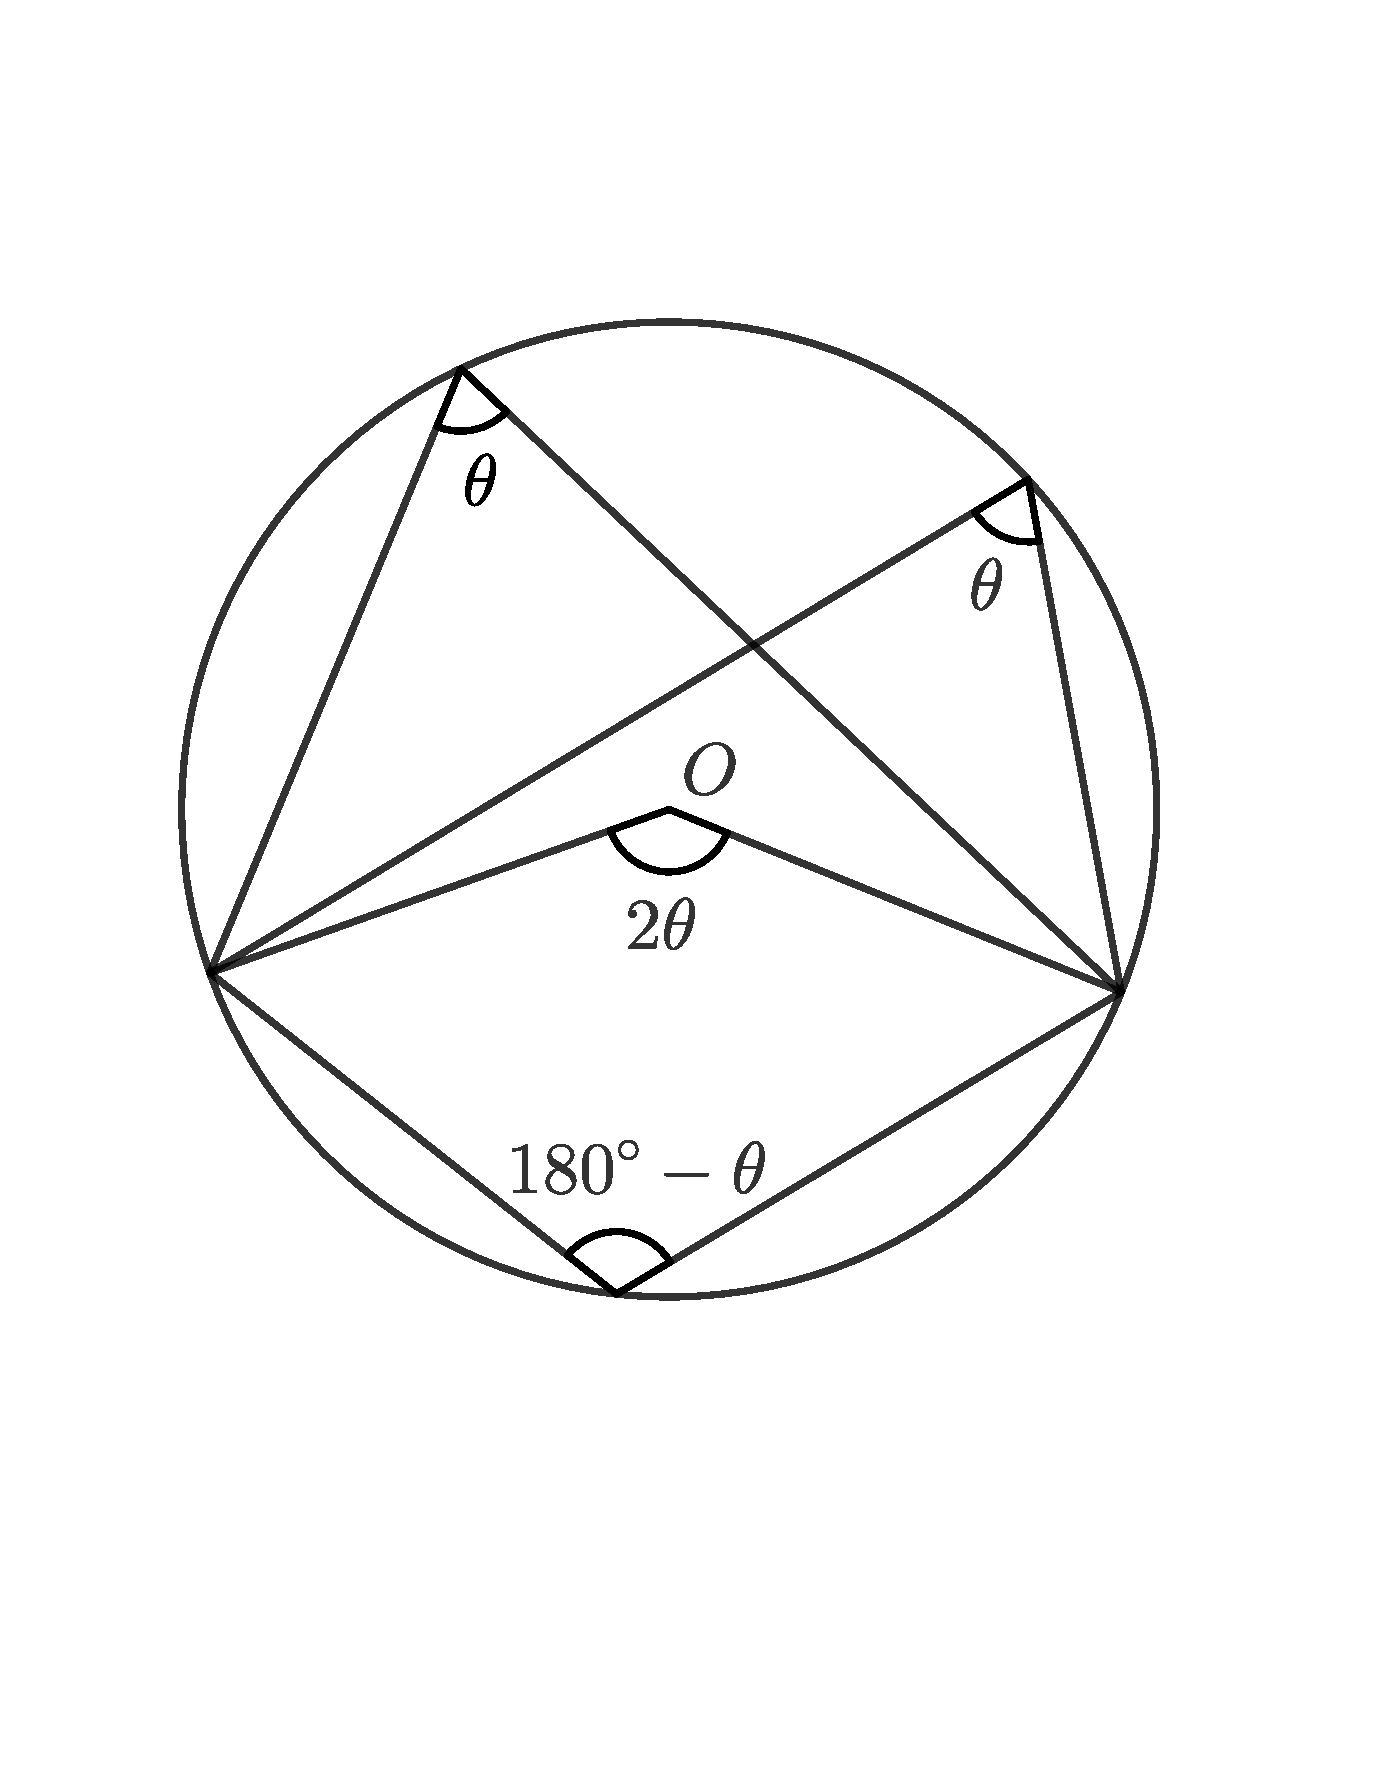
\includegraphics[clip,width=5cm]{figures/inscribed-angle.pdf}

\subsection{接弦定理}
図の角が等しい。
比較的頻出。

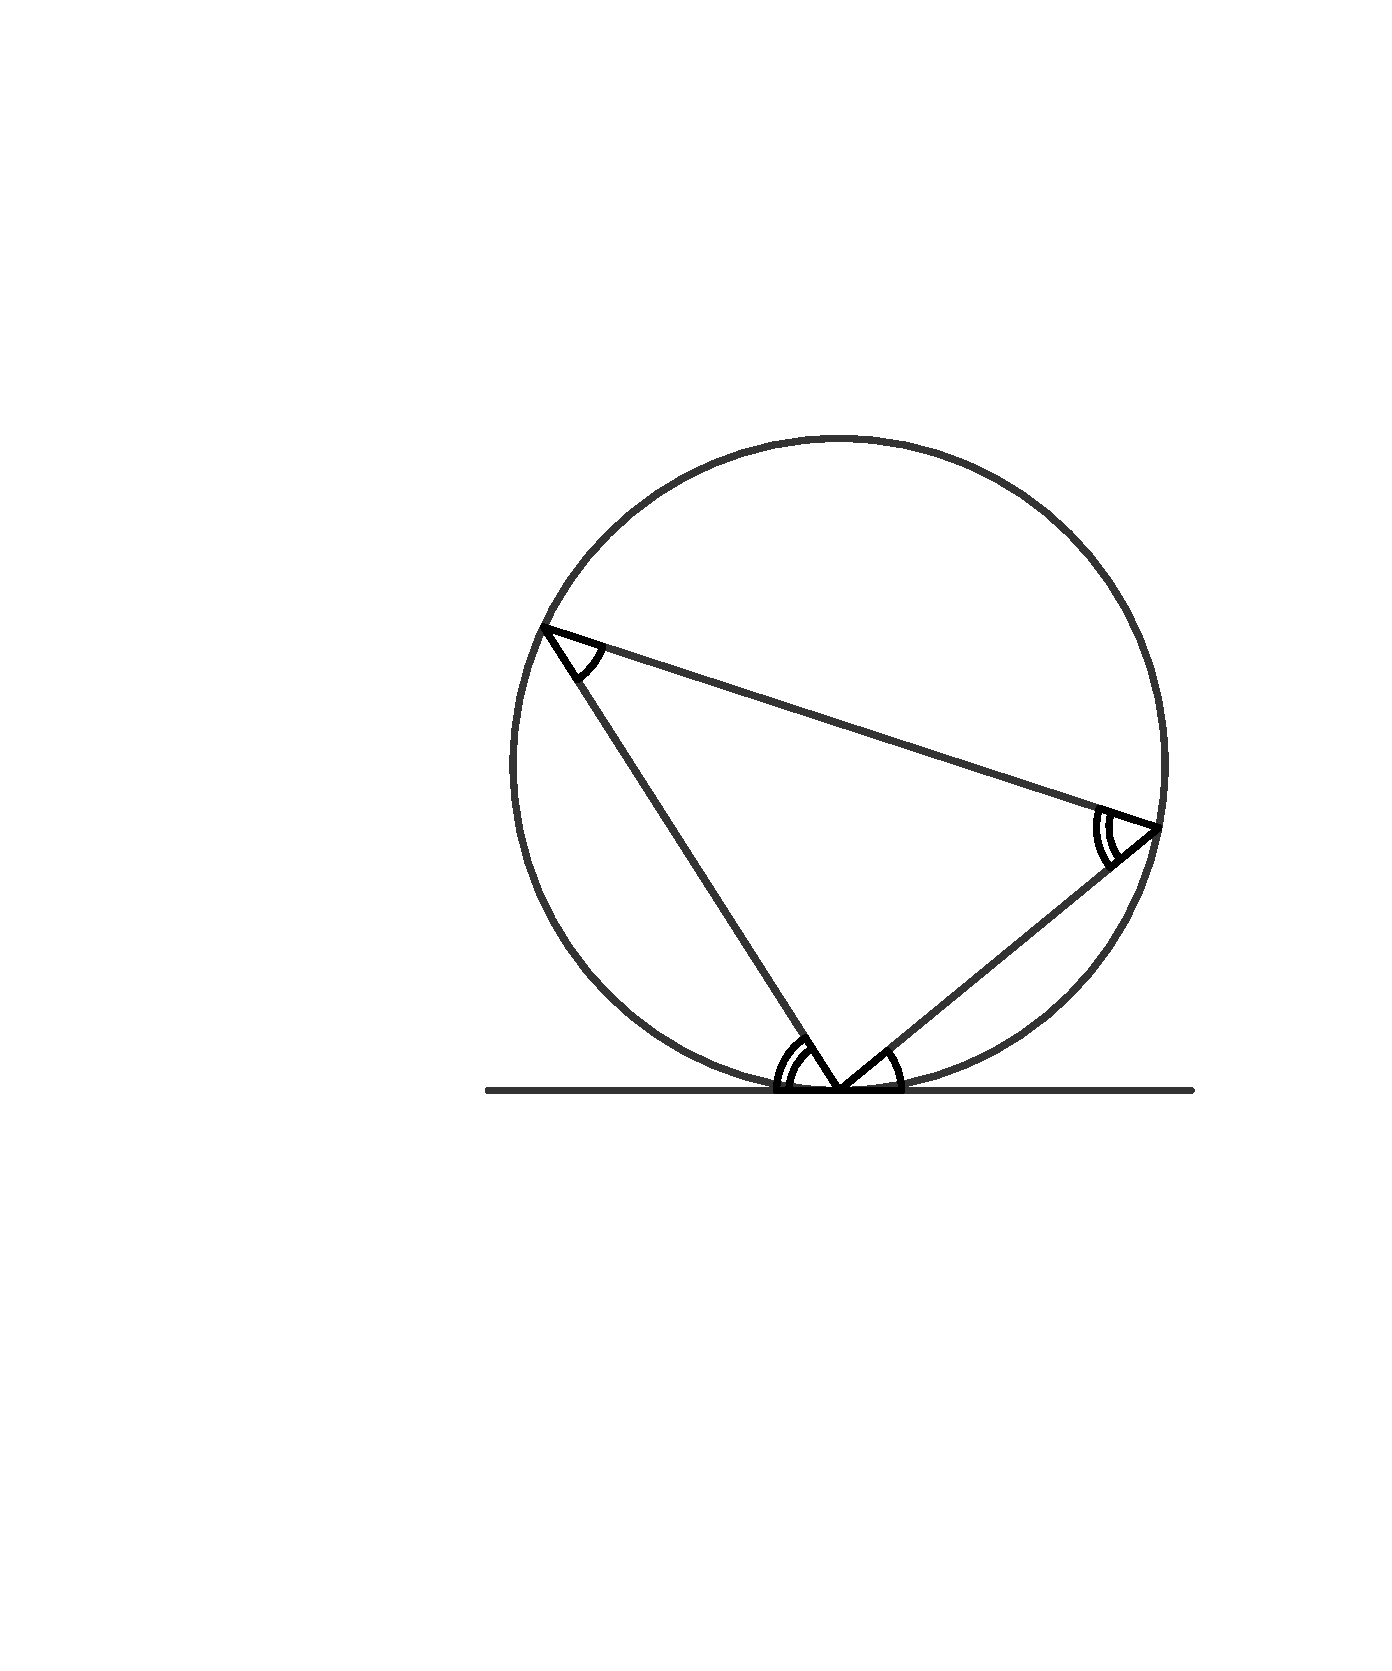
\includegraphics[clip,width=5cm]{figures/setsugen.pdf}

\subsection{方べきの定理}
よく出てくる。
\begin{itemize}
    \item $AE\times ED=BE\times EC$
    \item $AB^2=AC\times AD = AE \times AF$
\end{itemize}

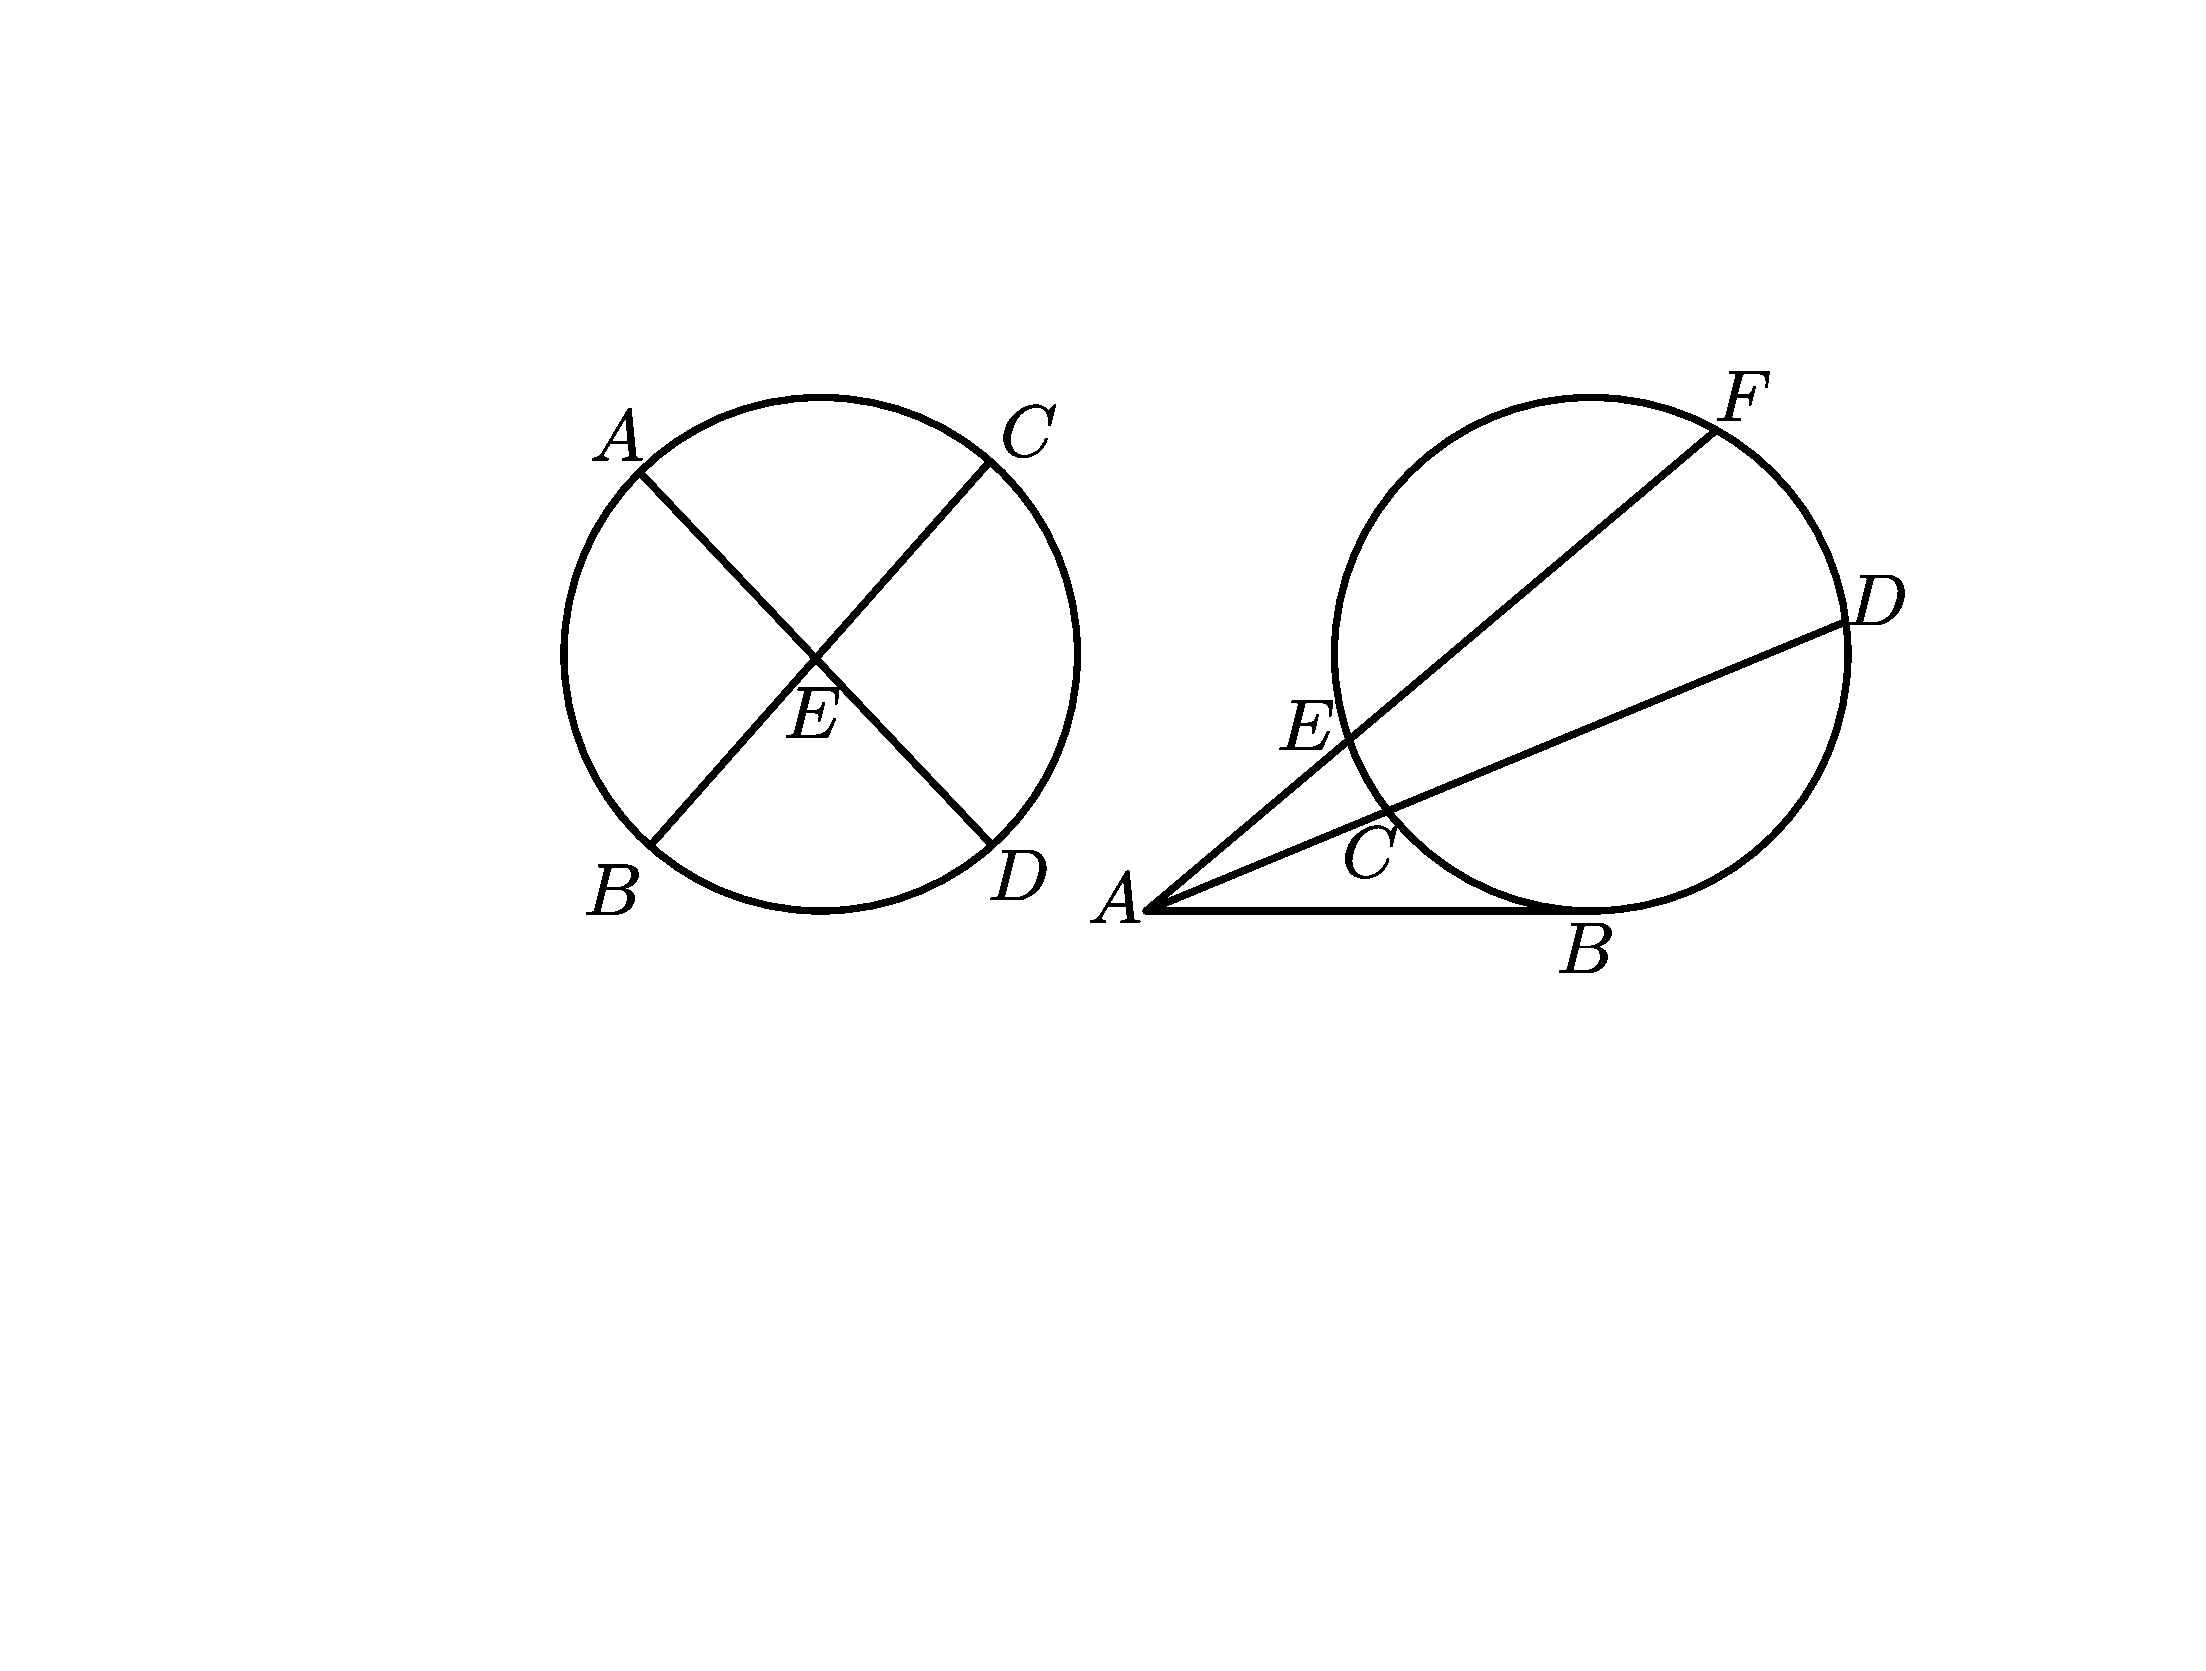
\includegraphics[clip,height=5cm]{figures/houbeki.pdf}

\subsection{共円な4点}
同一円周上にある4点のこと。
\begin{itemize}
    \item 相似
    \item 円周角の逆
    \item 方べきの逆
\end{itemize}
逆等を使って見つける。
見つけたら、その円を描いてみることで発見できることもあったりなかったりする。

\subsection{チェバの定理・メネラウスの定理}
使いどころが多いが、運用が難しい。
\begin{itemize}
    \item $\displaystyle \frac{AD}{DB} \times \frac{BE}{EC} \times \frac{CF}{FA} = 1$
    \item $\displaystyle \frac{GJ}{JH} \times \frac{HK}{KI} \times \frac{IL}{LG} = 1$
\end{itemize}

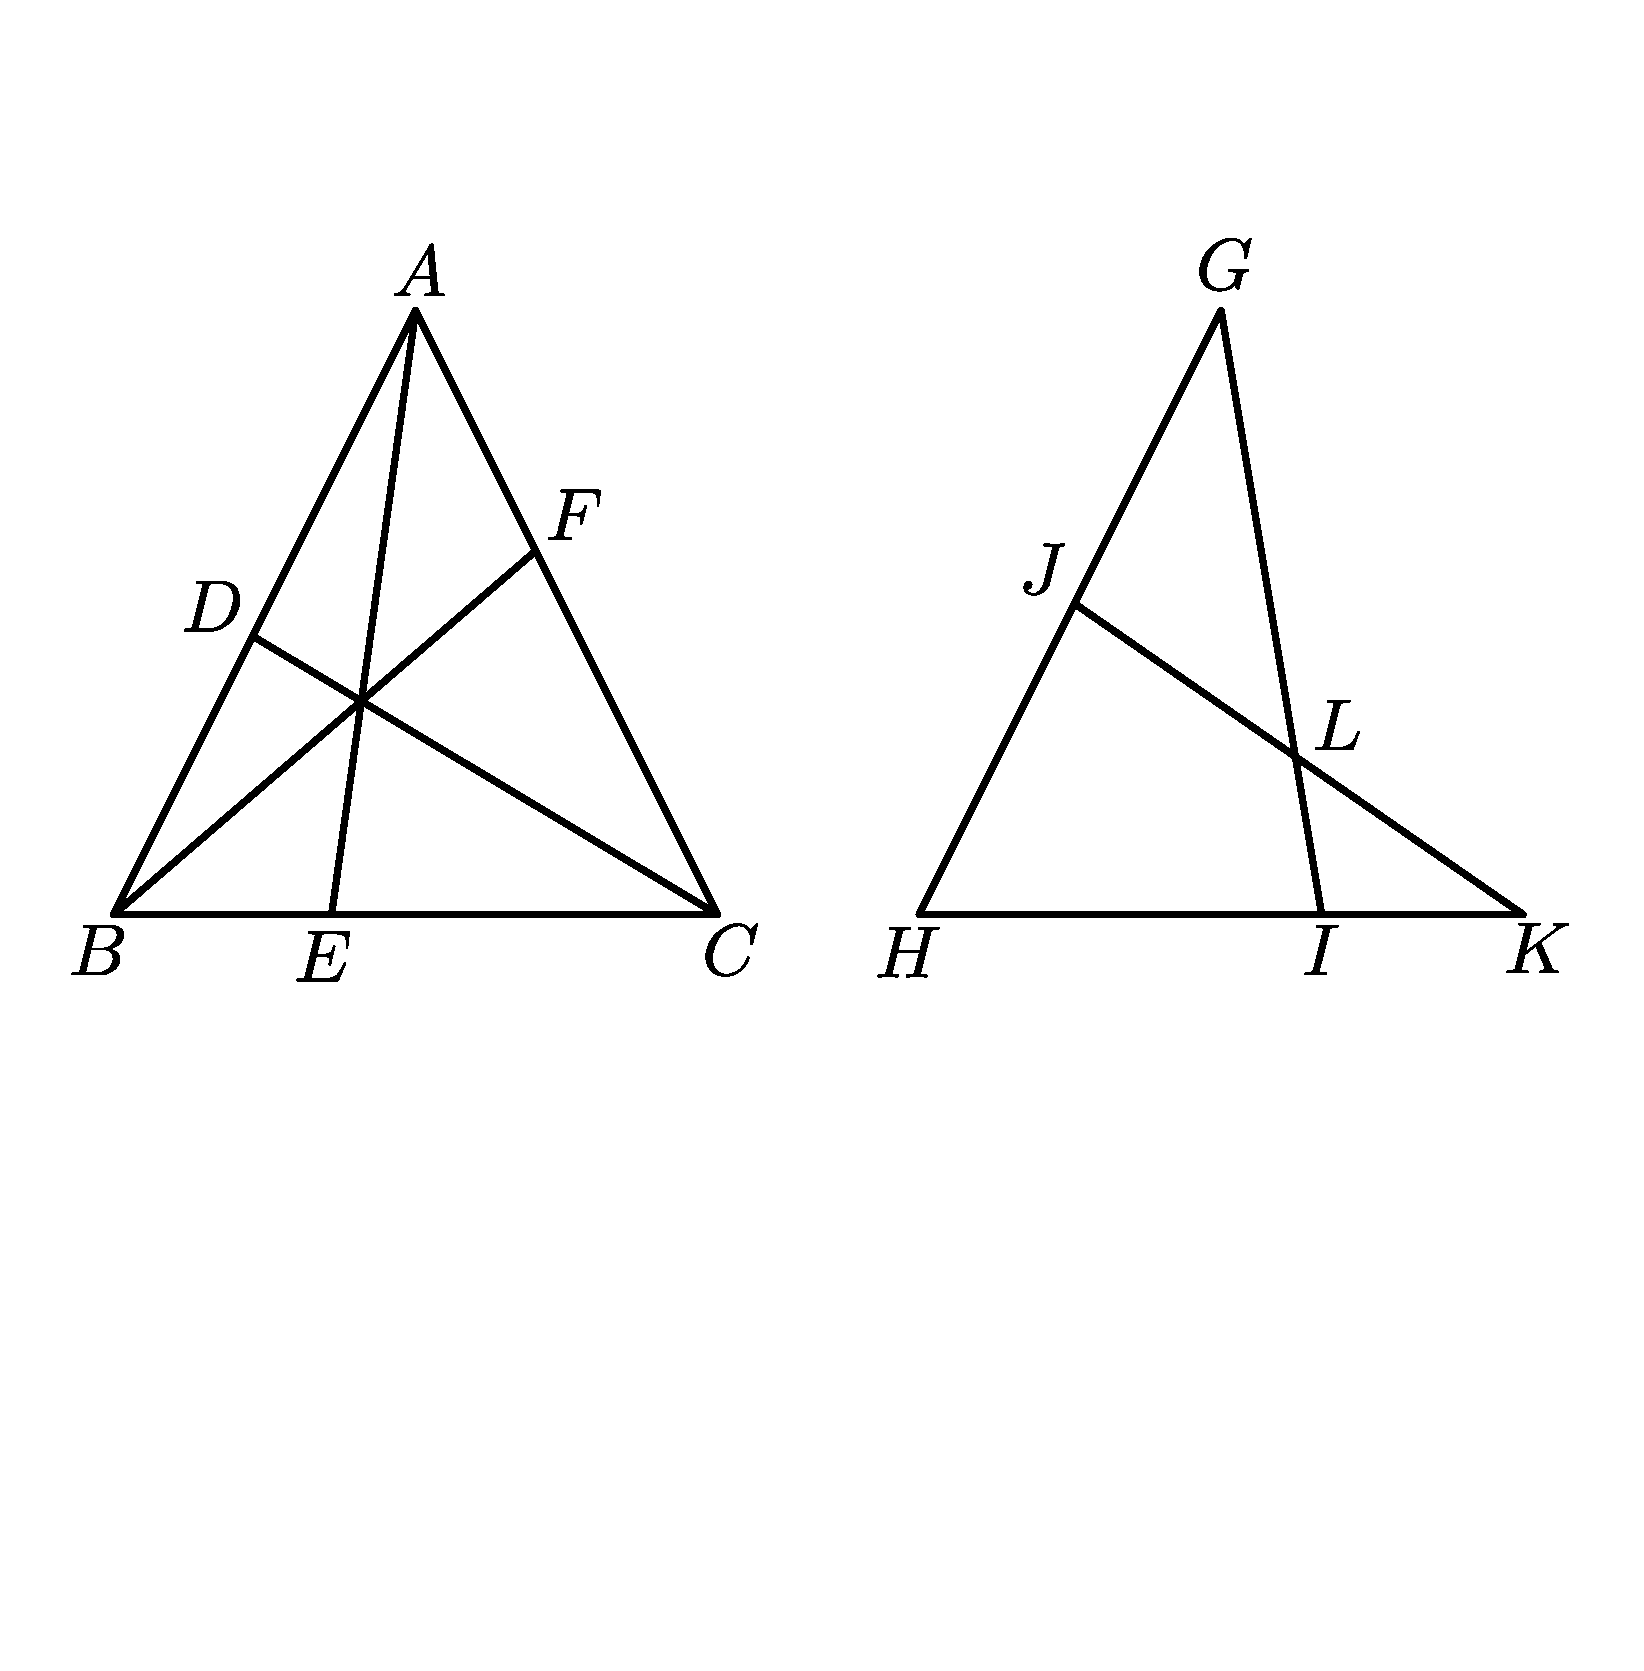
\includegraphics[clip,height=5cm]{figures/Ceva_Menelaus.pdf}

\subsection{Angle-chase}
\begin{itemize}
    \item 相似
    \item 円周角の定理
    \item 同位角・錯覚
\end{itemize}

等を使って同じ角度を追いかけていく。

$\rightarrow$新たな相似、合同、共円な4点が見つかるかもしれない。

\subsection{角の二等分線}
\begin{itemize}
    \item $AB:BC=BD:DC=BE:EC$
\end{itemize}

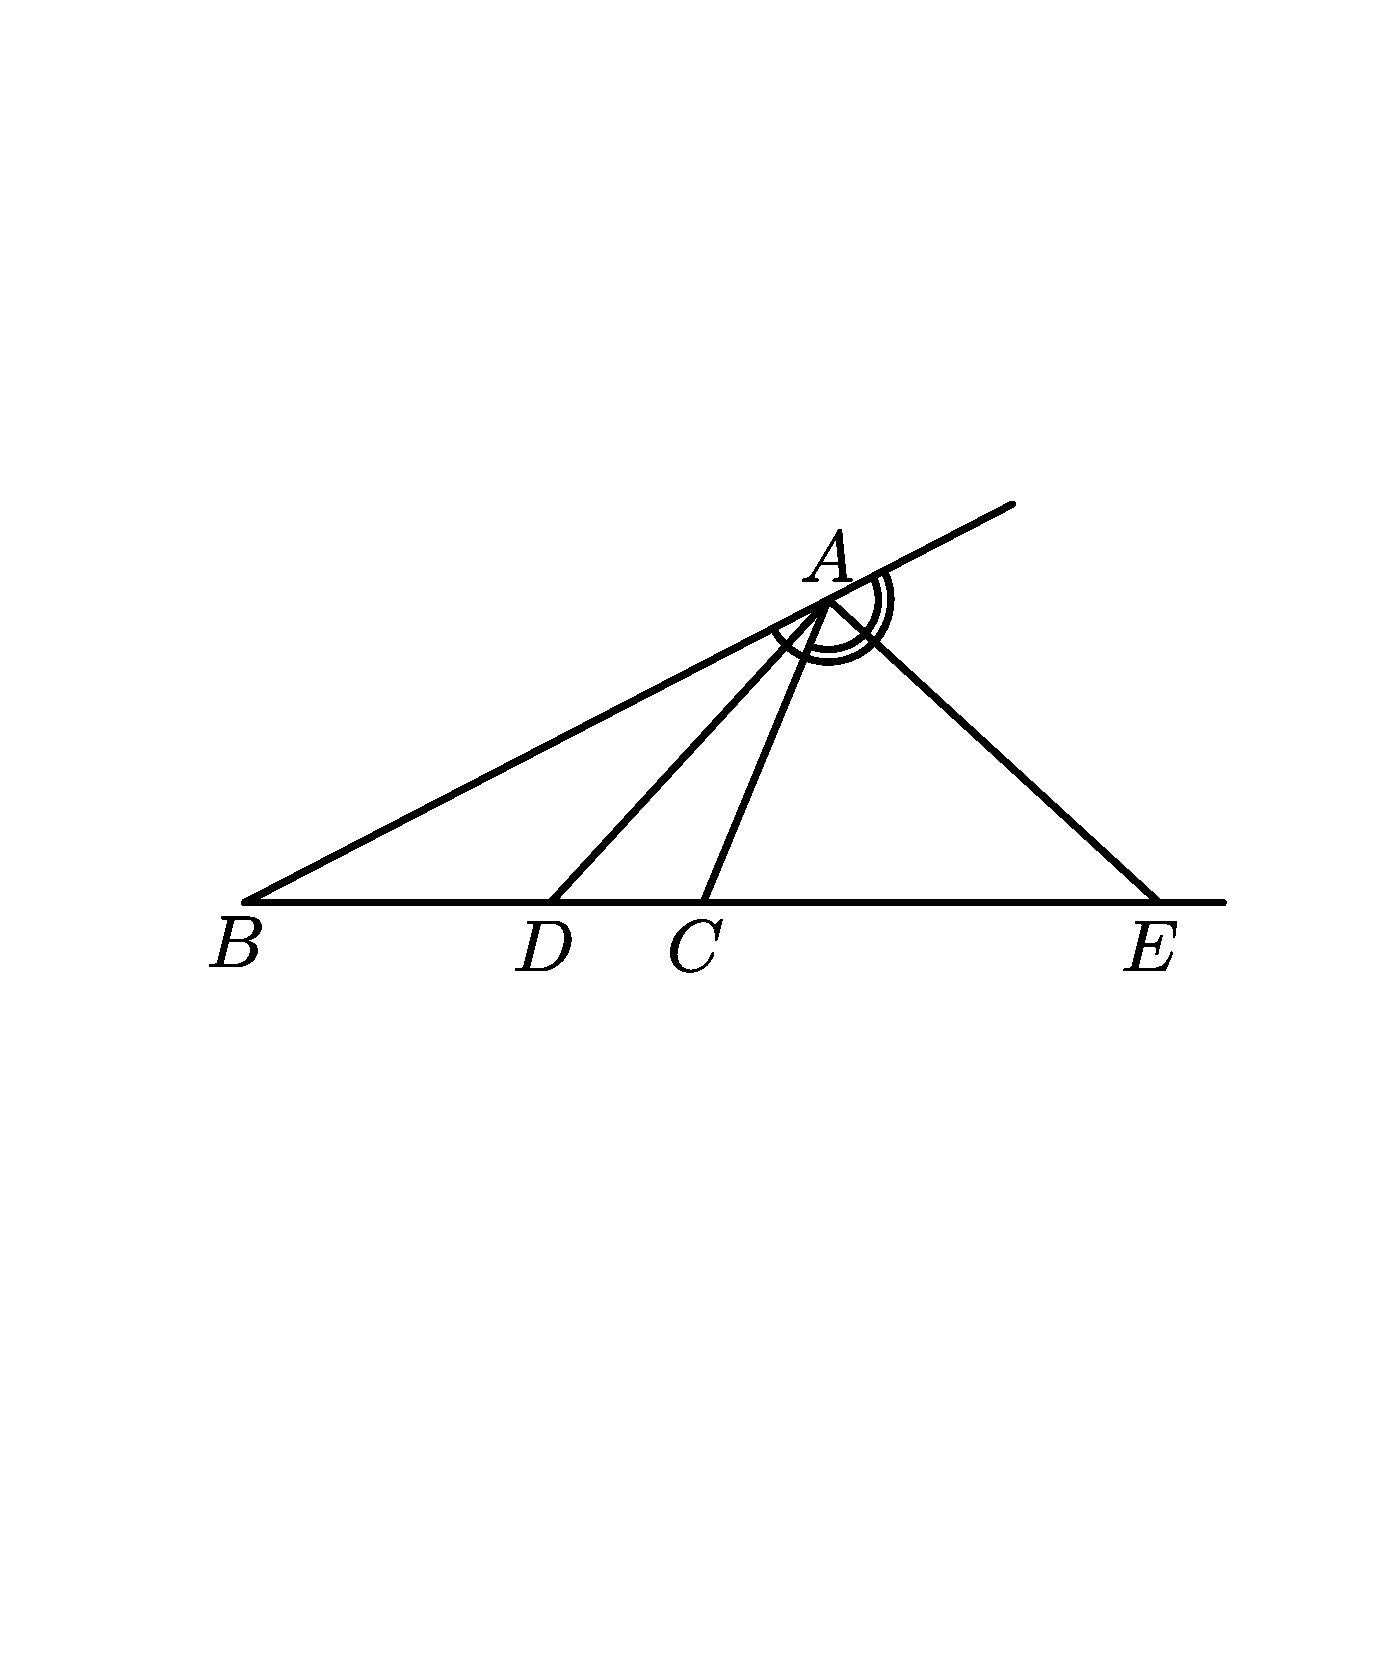
\includegraphics[clip,width=6cm]{figures/nitobun.pdf}

\subsection{中線定理}
\begin{itemize}
    \item $AB^2+AC^2=2\left(AM^2+BM^2\right)$
\end{itemize}

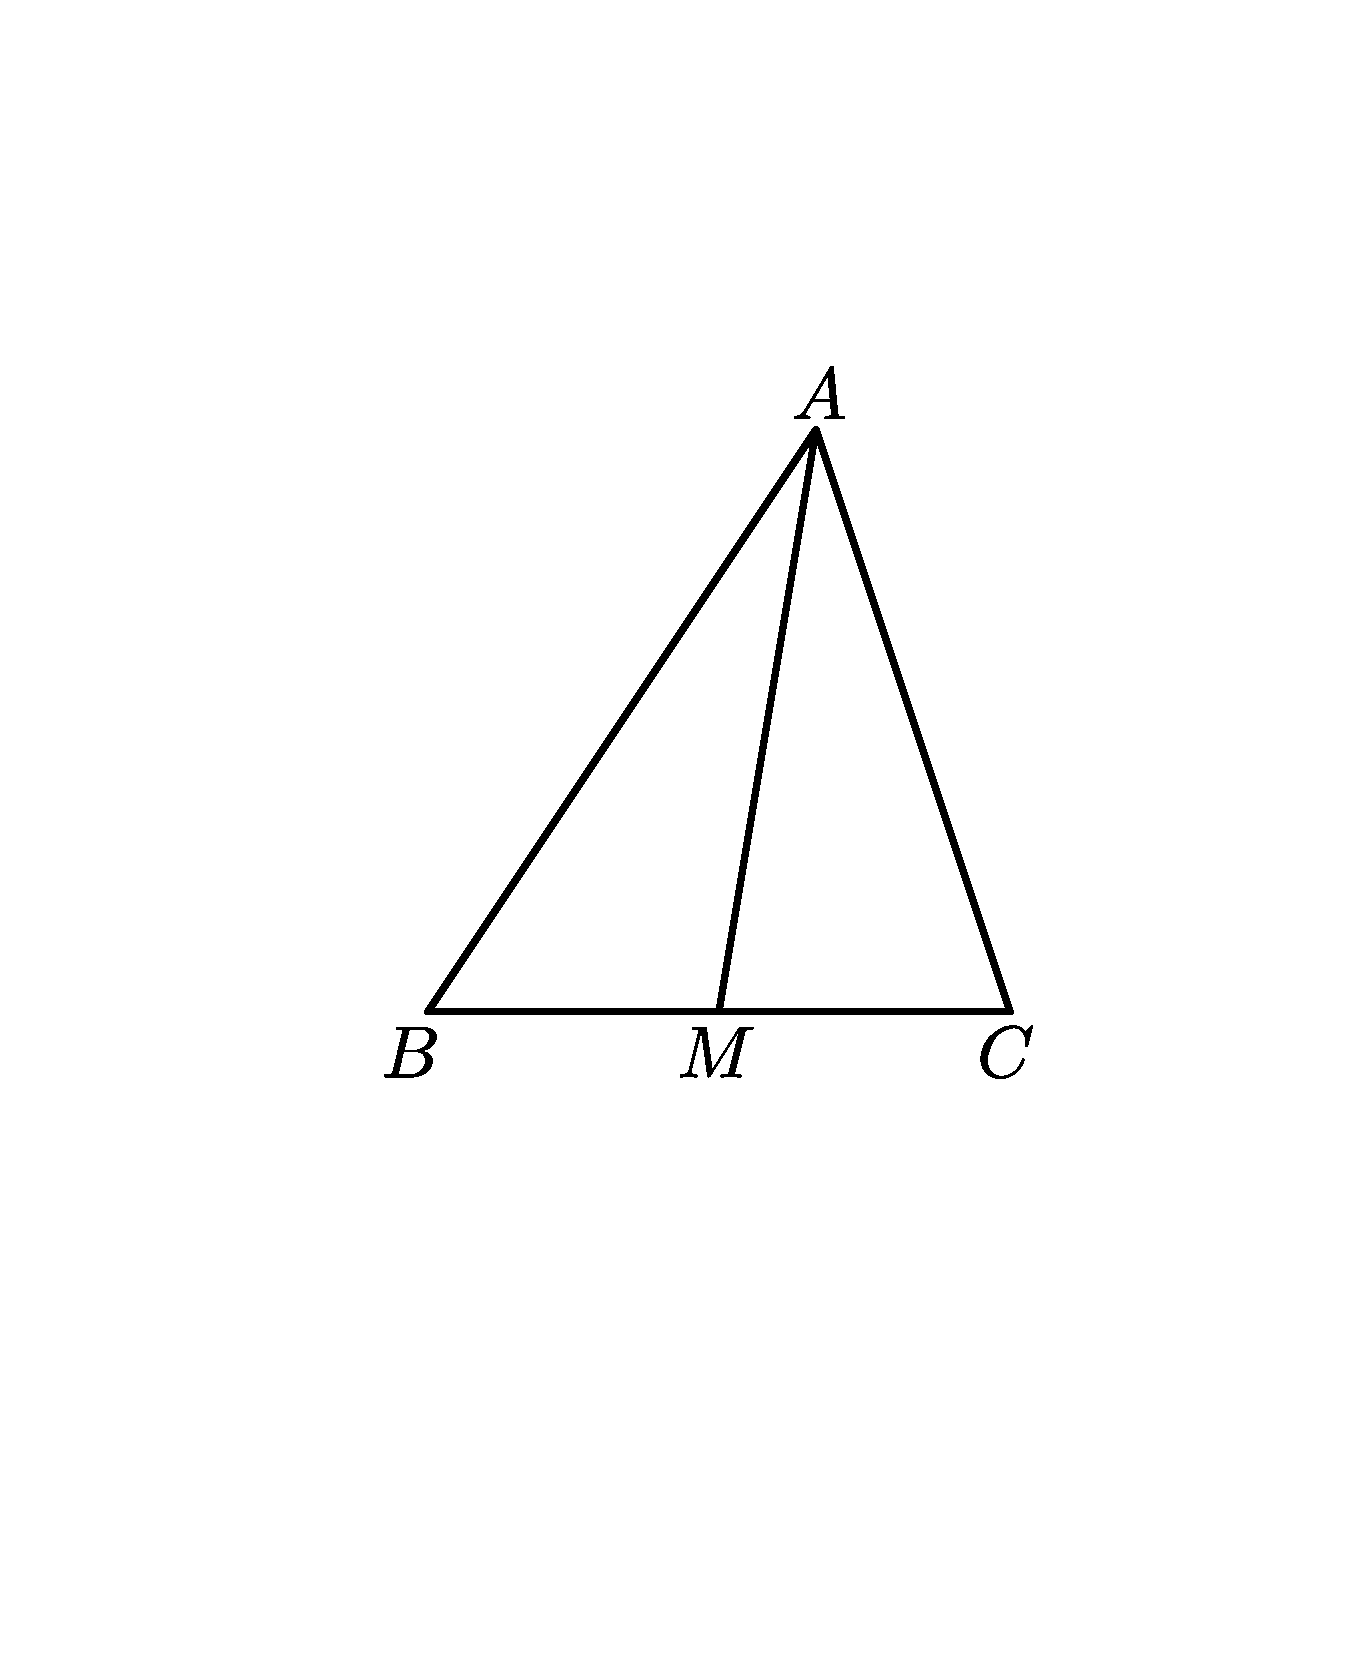
\includegraphics[clip,height=5cm]{figures/chusen.pdf}

\subsection{補助線}
\begin{itemize}
    \item 基本事項が使えるように引く
    \item 二等辺三角形をいっぱい作る
\end{itemize}
等、やみくもに引かず、
うまくいくようにやるのが大事

\subsection{三角形の五心}

これらの点が問題に出ていなくても、これらを考えることで問題が解きやすくなることがある。
例えば、直線上に垂心があることを示すことで、二直線が直交することを示すことができる。

\begin{itemize}
    \item 内心$I$
    \begin{itemize}
        \item $A$から接点までの距離は$\displaystyle \frac{AB+CA-BC}{2}$
    \end{itemize}
    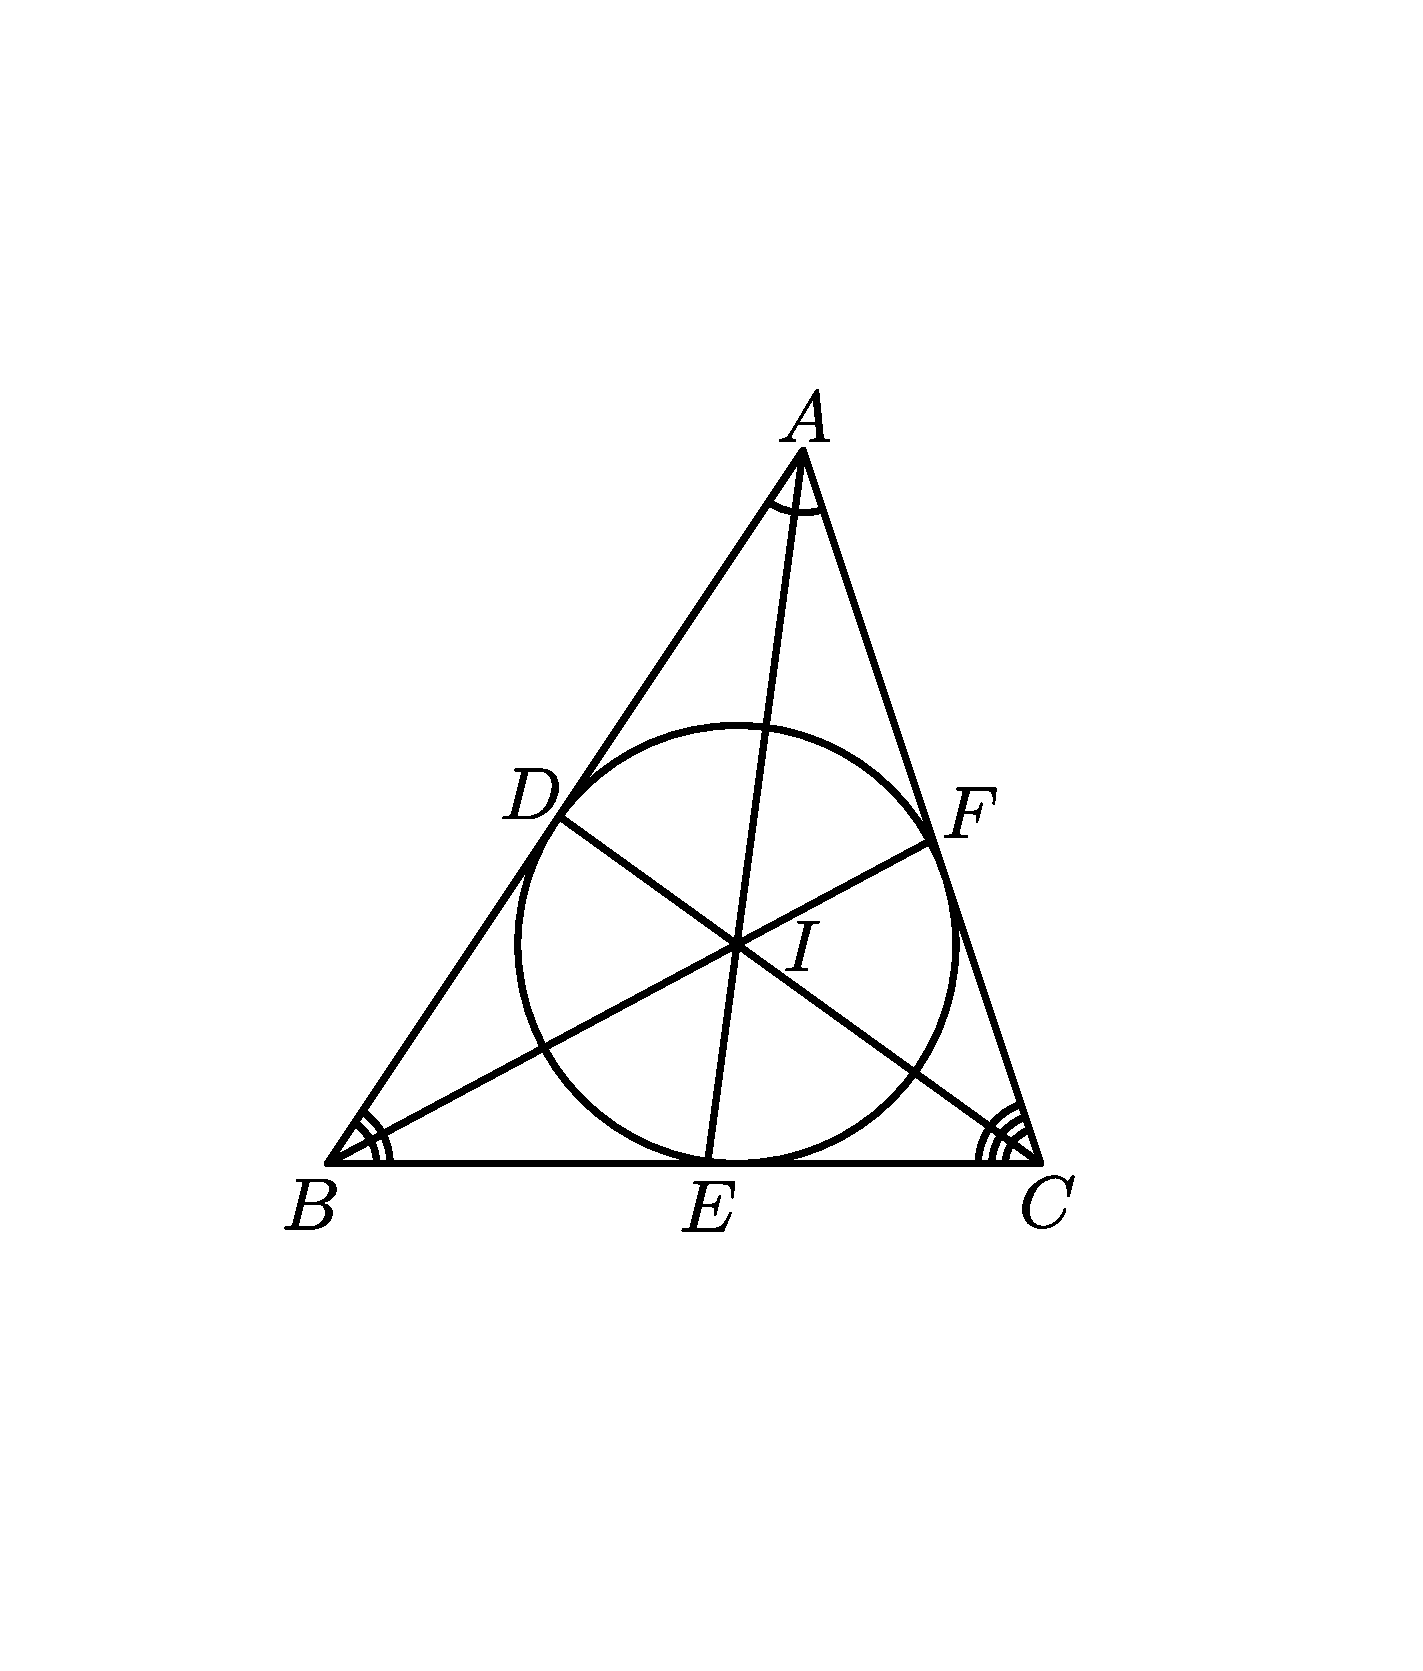
\includegraphics[clip,height=5cm]{figures/Naishin.pdf}

    \item 傍心$I_A$
    \begin{itemize}
        \item $A$から接点までの距離は$\displaystyle \frac{AB+BC+CA}{2}$
    \end{itemize}
    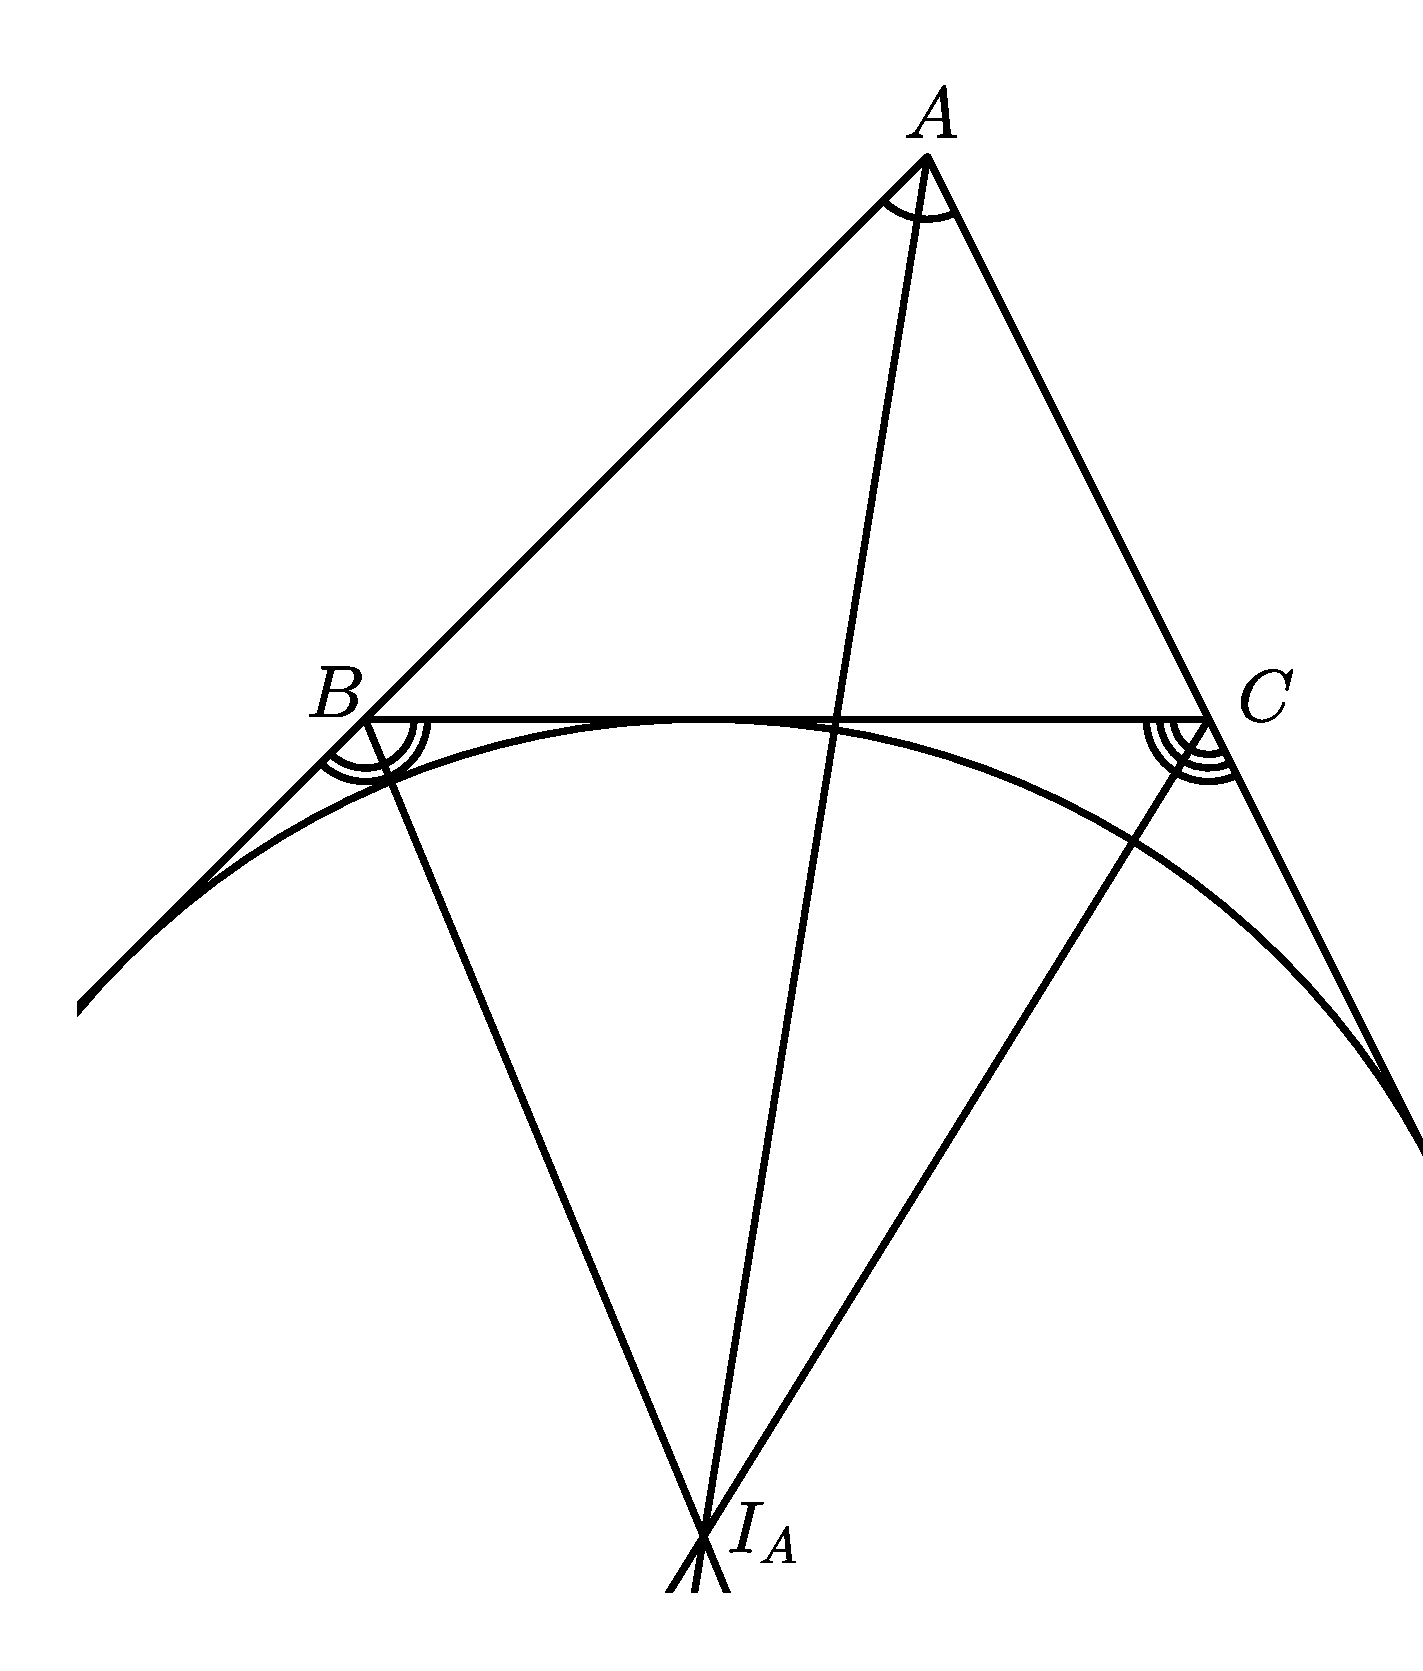
\includegraphics[clip,height=5cm]{figures/Boushin.pdf}

    \item 重心$G$

    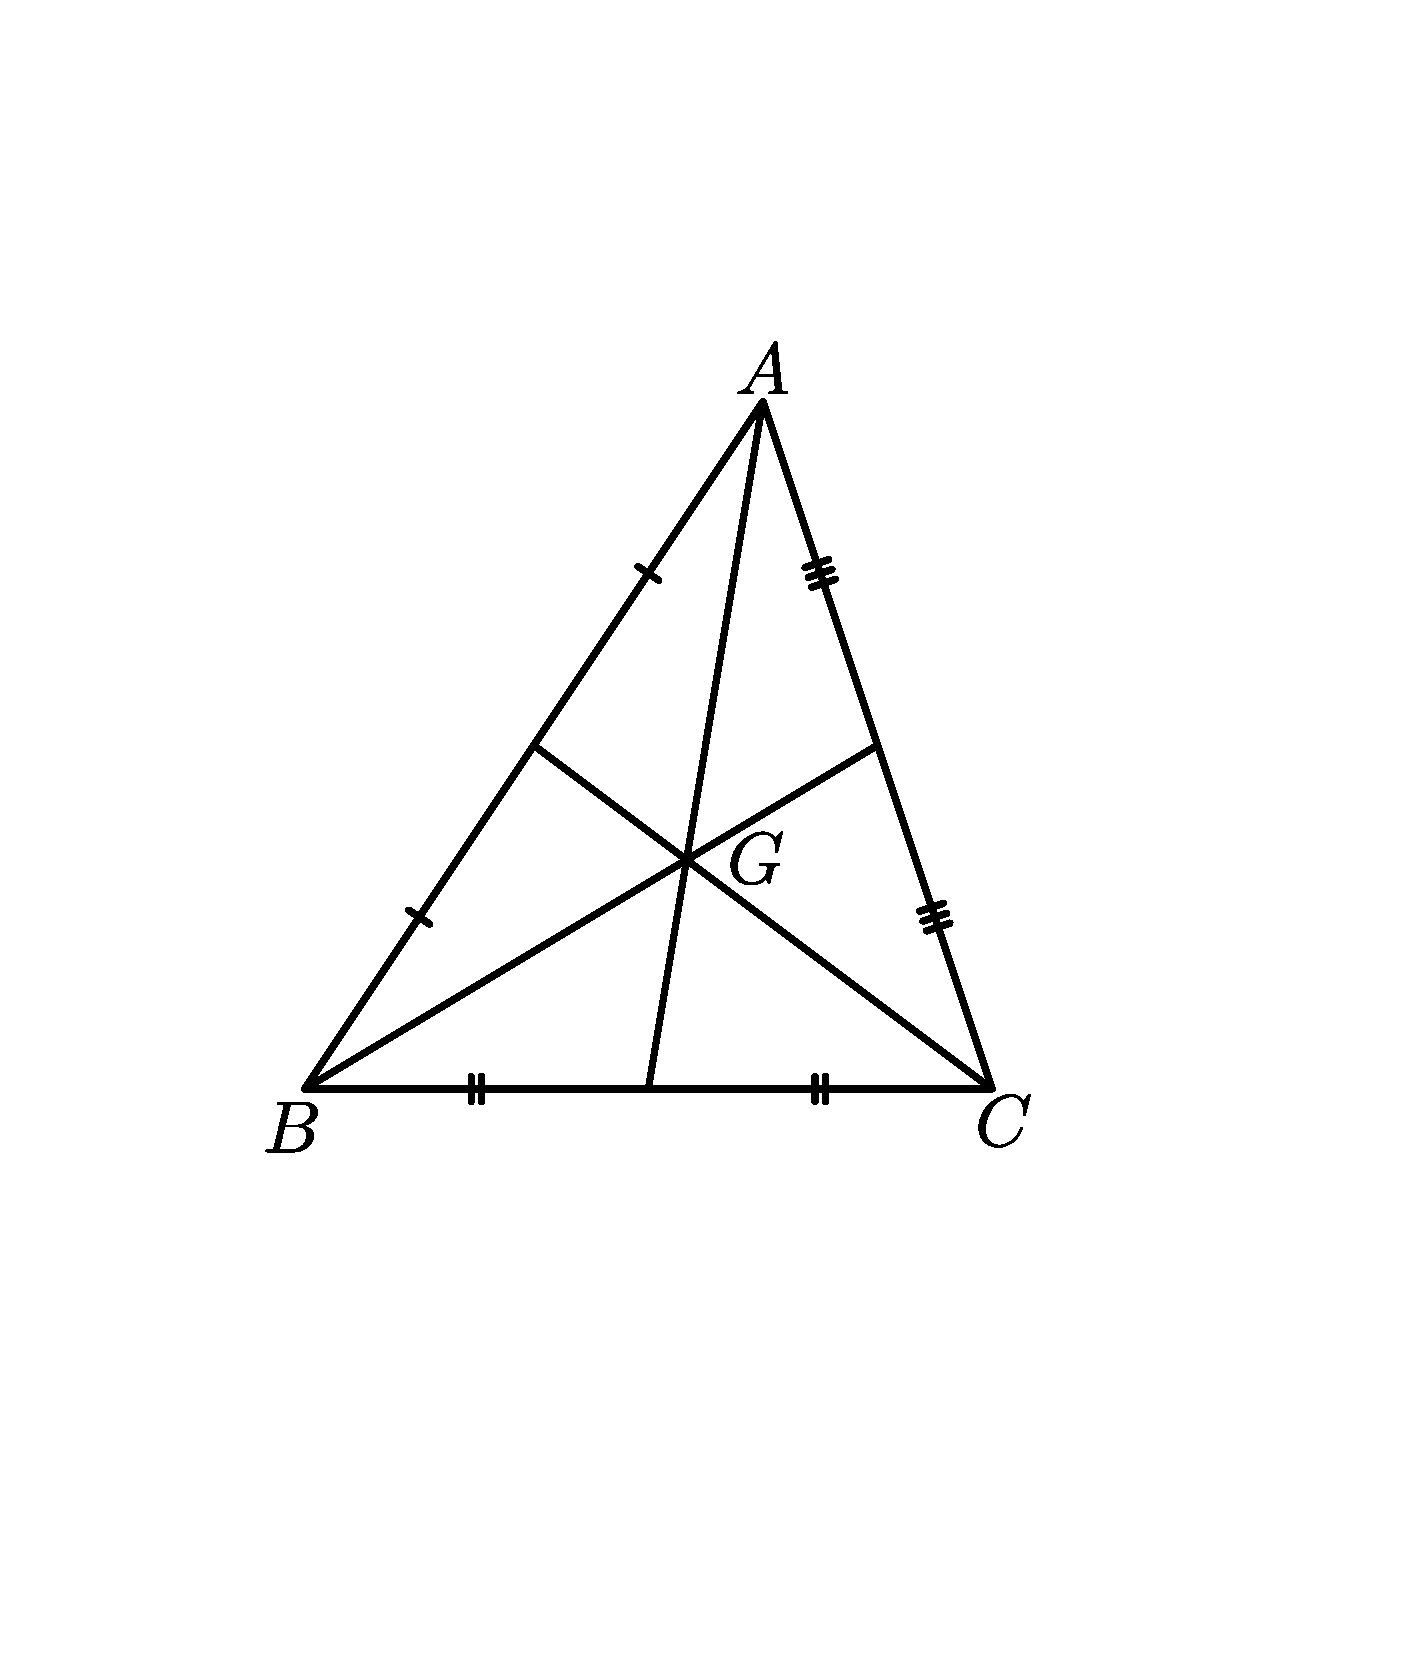
\includegraphics[clip,height=5cm]{figures/Jushin.pdf}

    \item 垂心$H$

    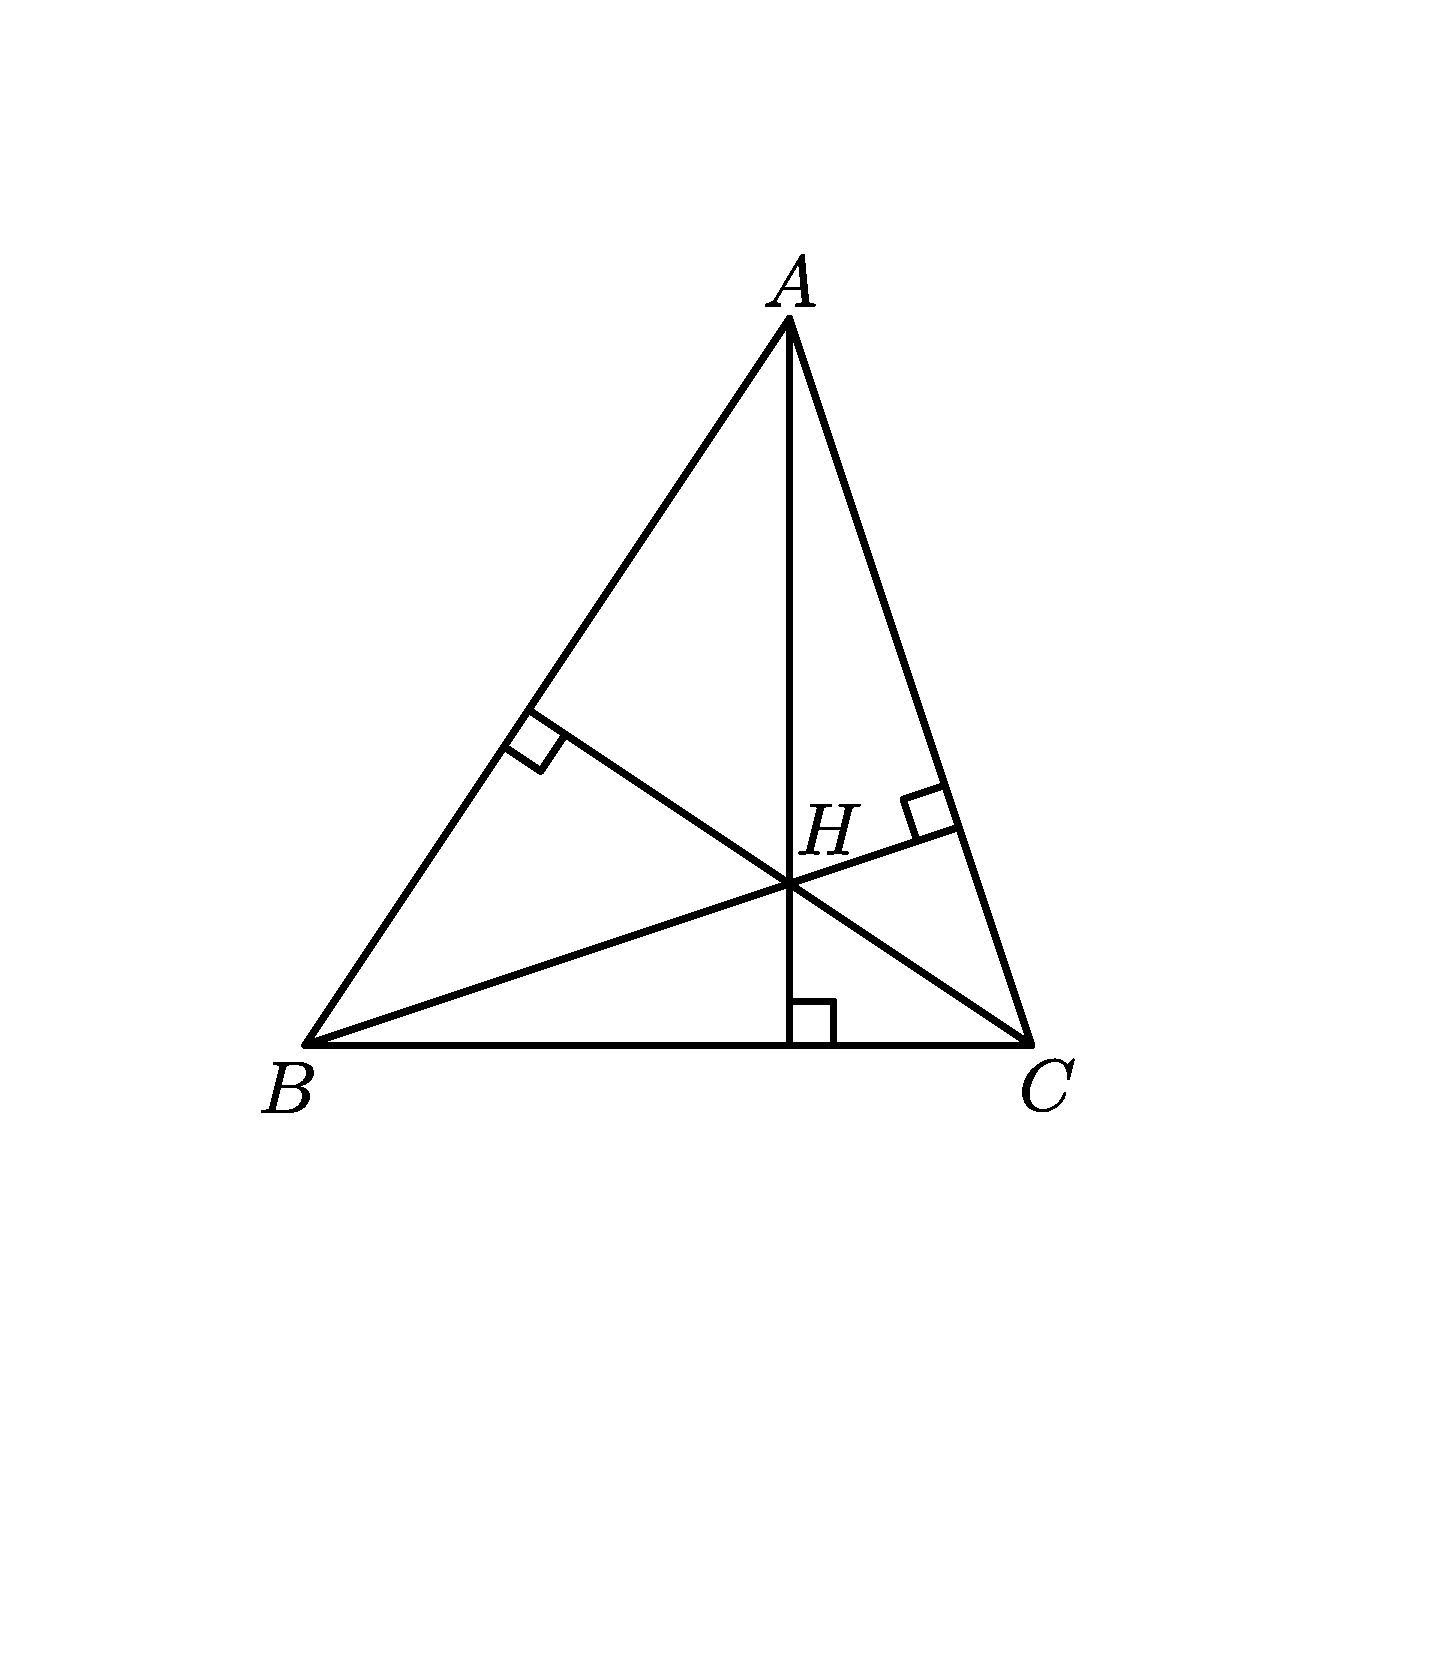
\includegraphics[clip,height=5cm]{figures/Suishin.pdf}

    \item 外心$O$

    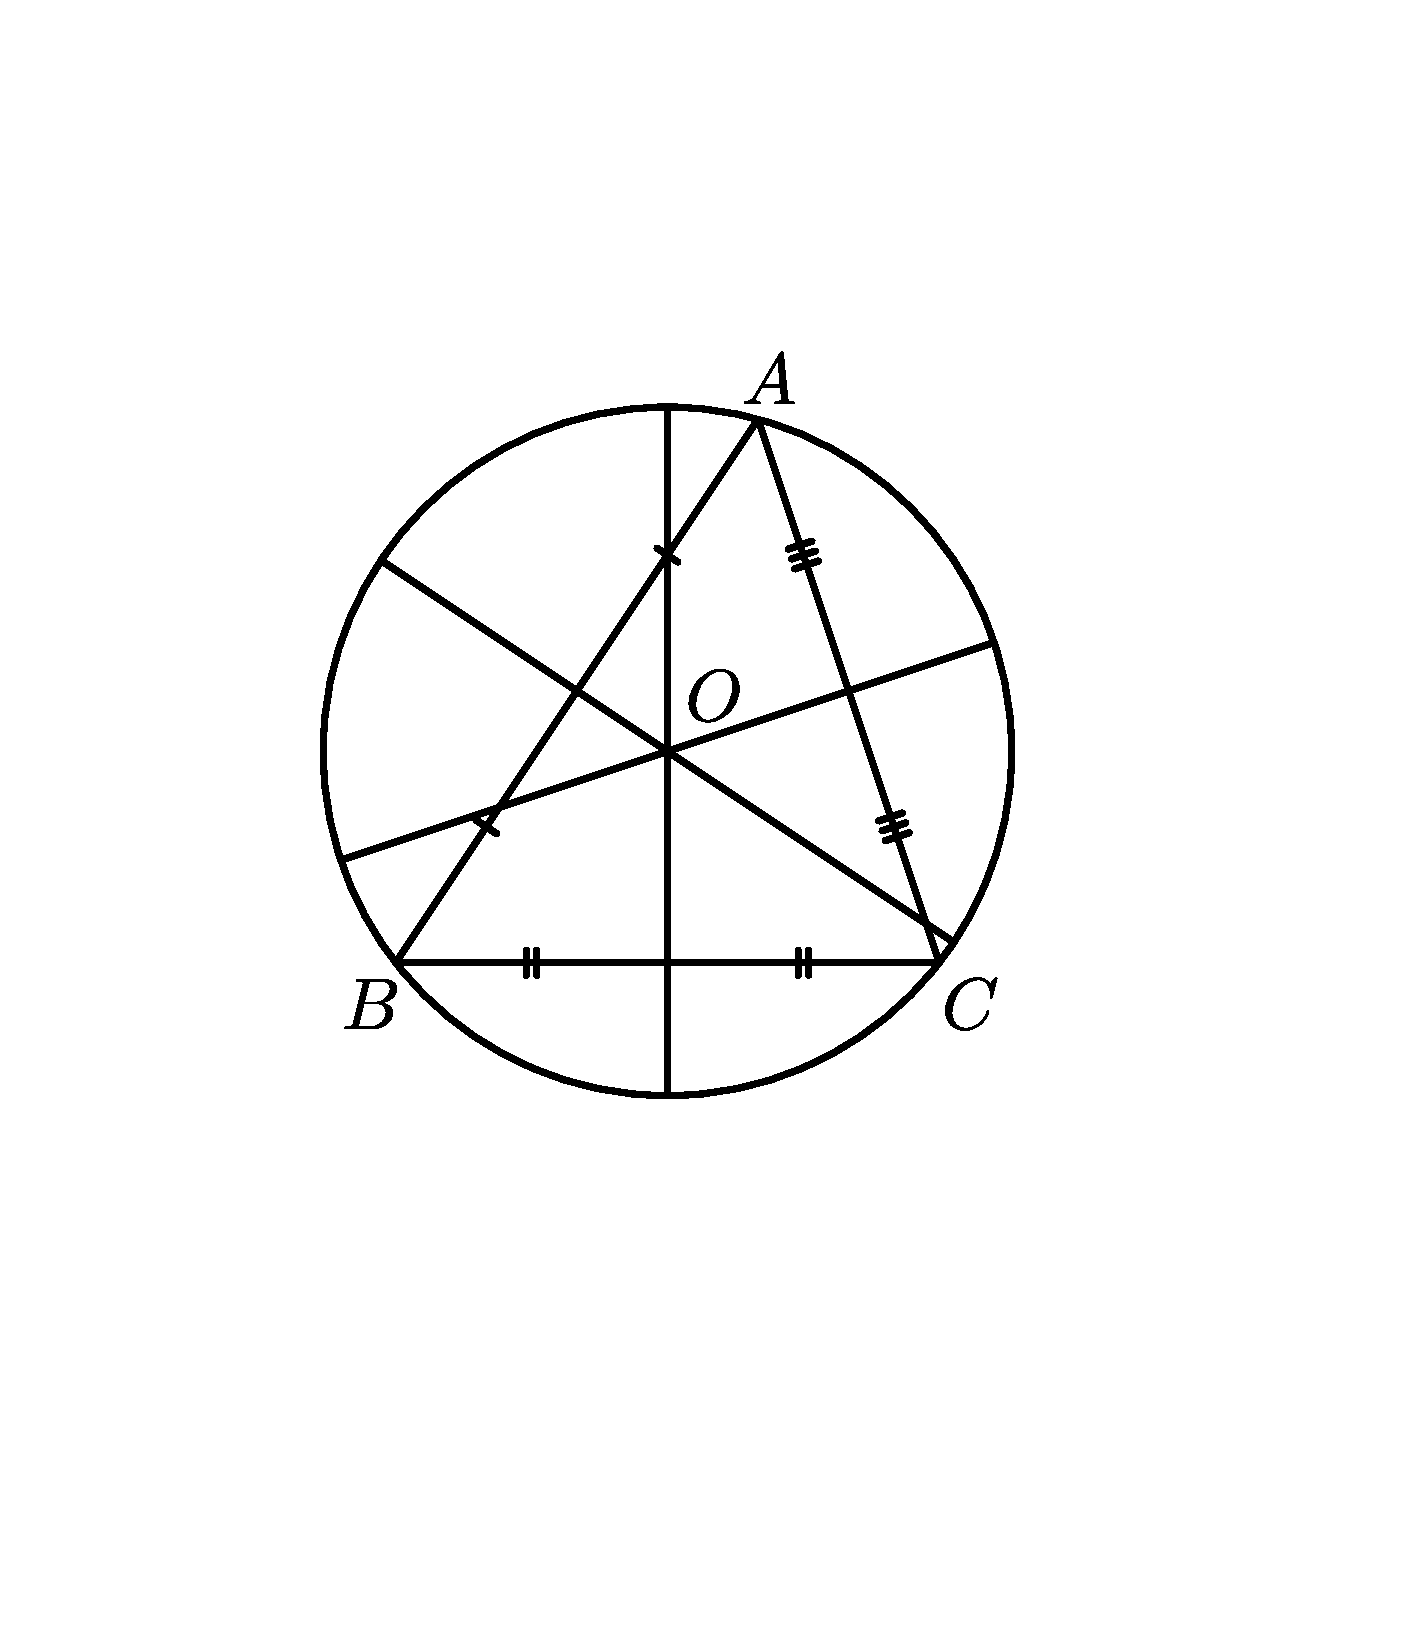
\includegraphics[clip,height=5cm]{figures/Gaishin.pdf}
\end{itemize}

\subsection{垂心について}
垂心は頂点から辺に引いた垂線の交点あるから、以下のような円がかける。
また、円周角の定理より、図に示した角が等しい。
このような性質から、垂心周りの角度を簡単に表すことができる。

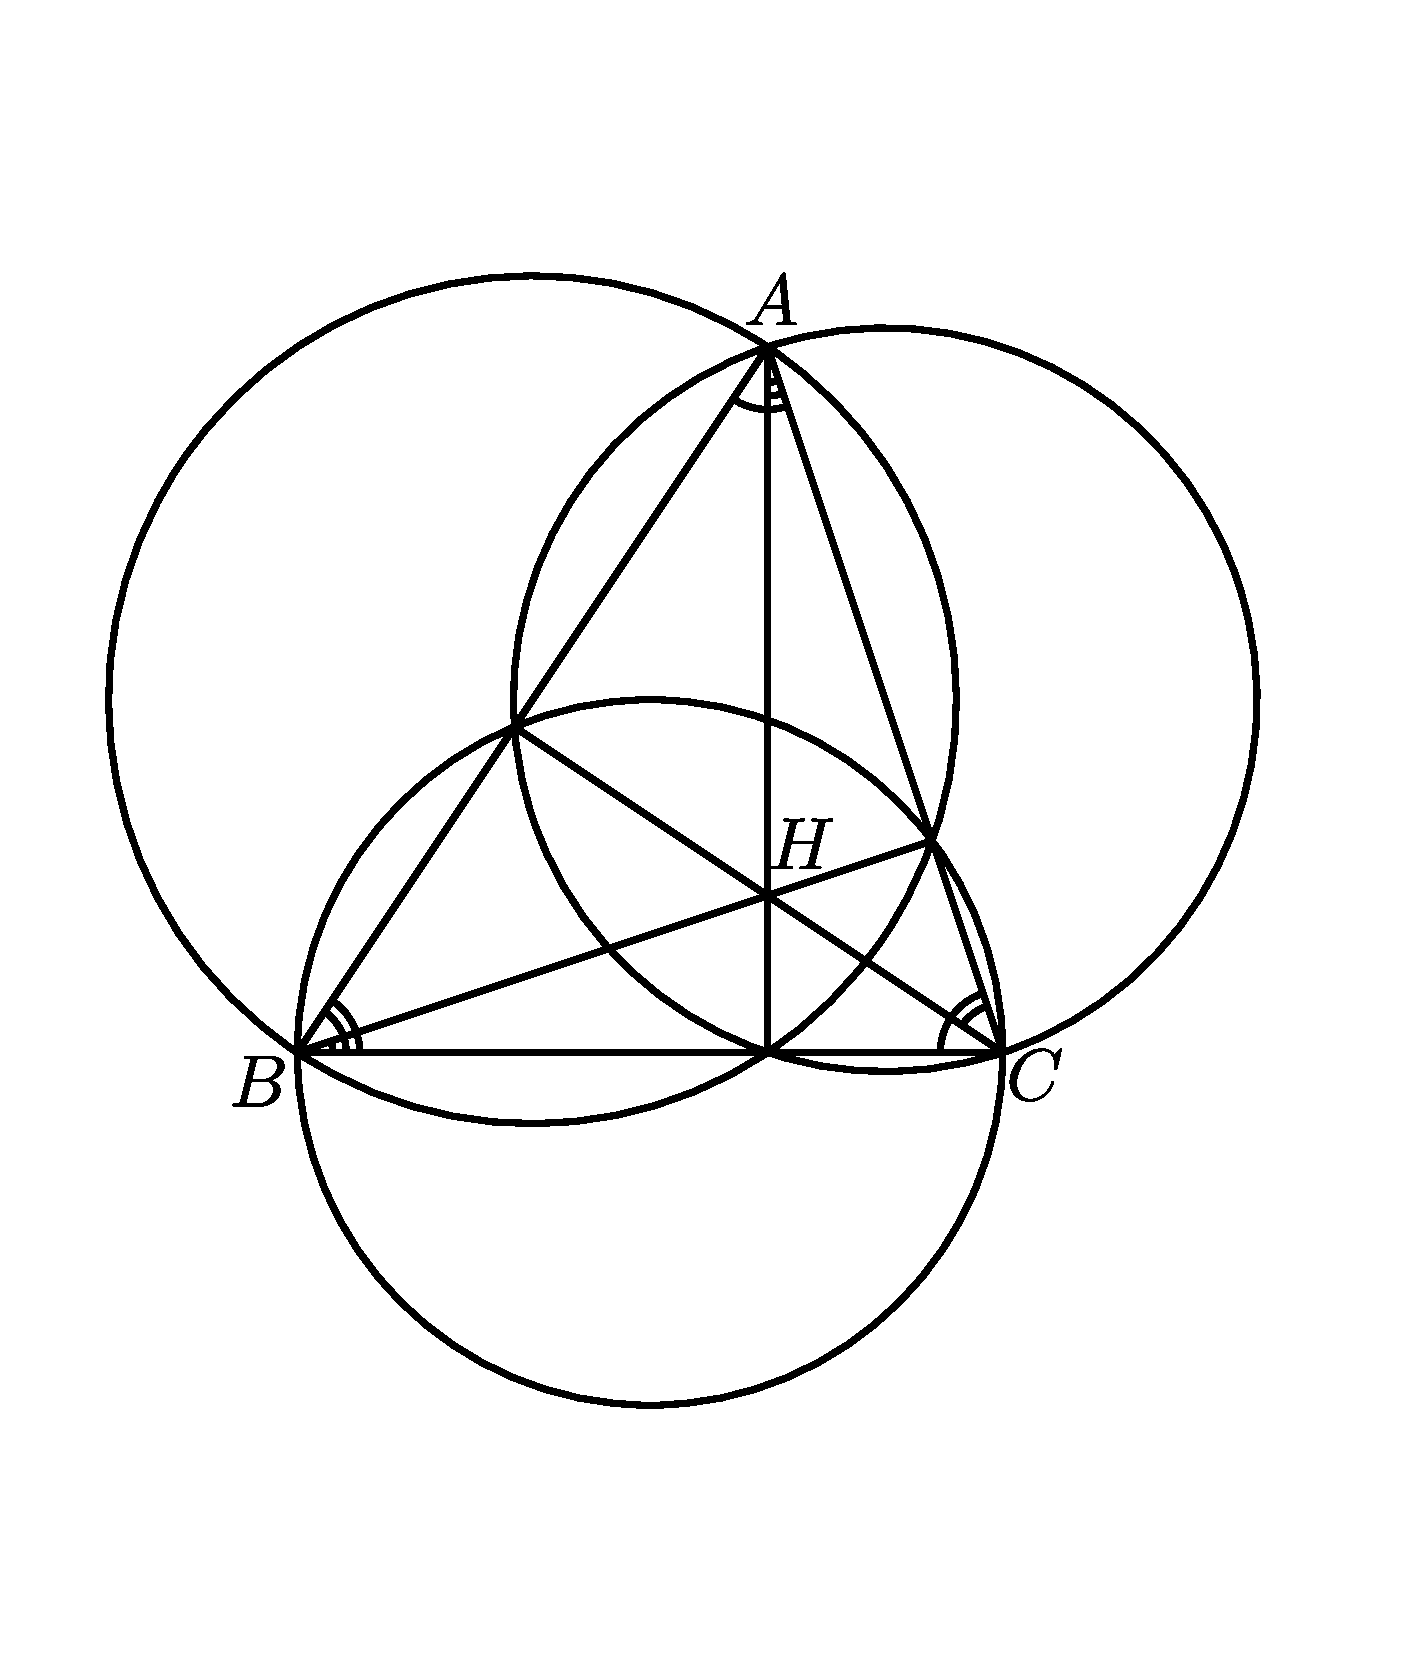
\includegraphics[clip,height=5cm]{figures/Suishin1.pdf}
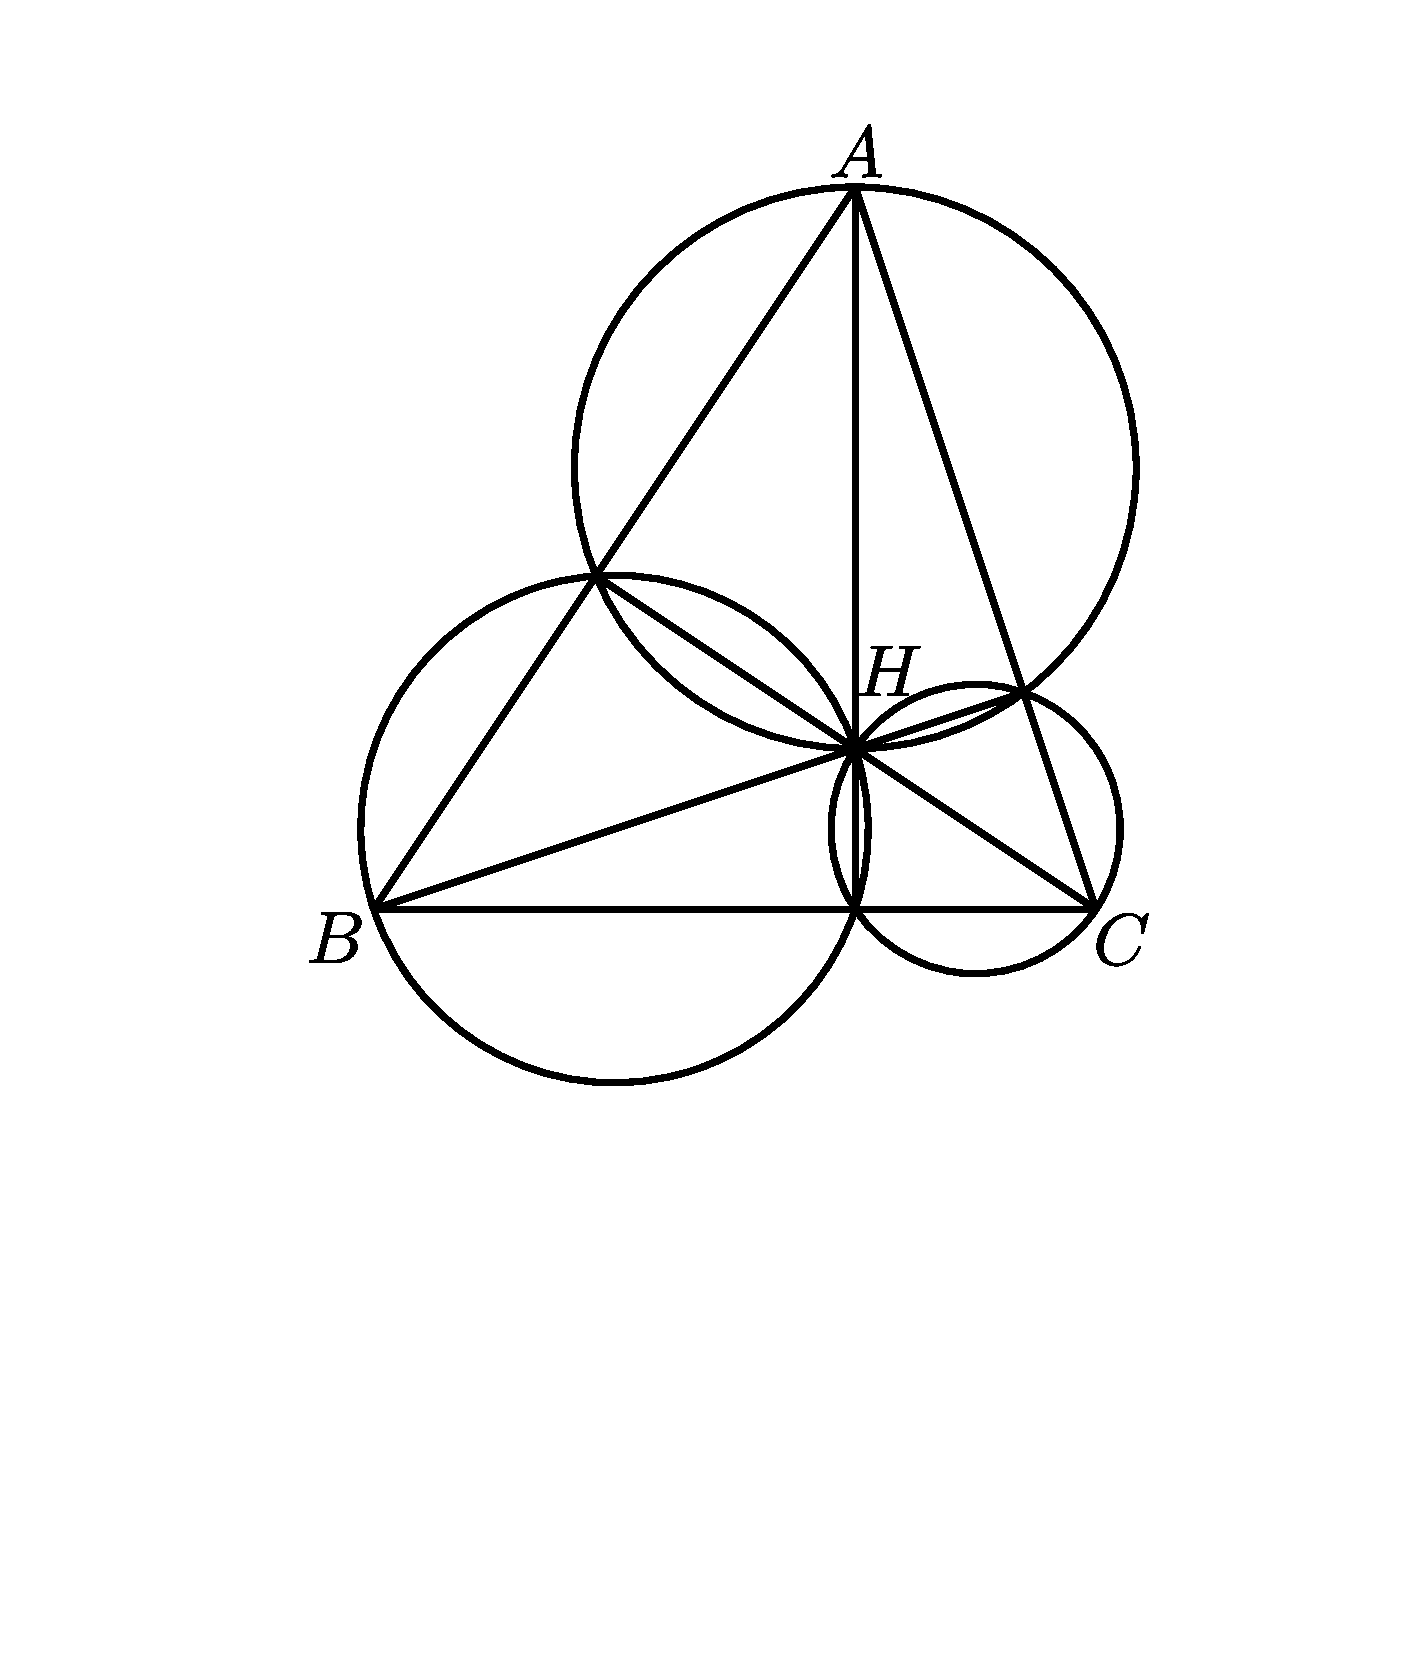
\includegraphics[clip,height=5cm]{figures/Suishin2.pdf}

\subsection{オイラー線}
三角形の垂心、重心、外心は同一直線状に存在し、この直線をオイラー線という。

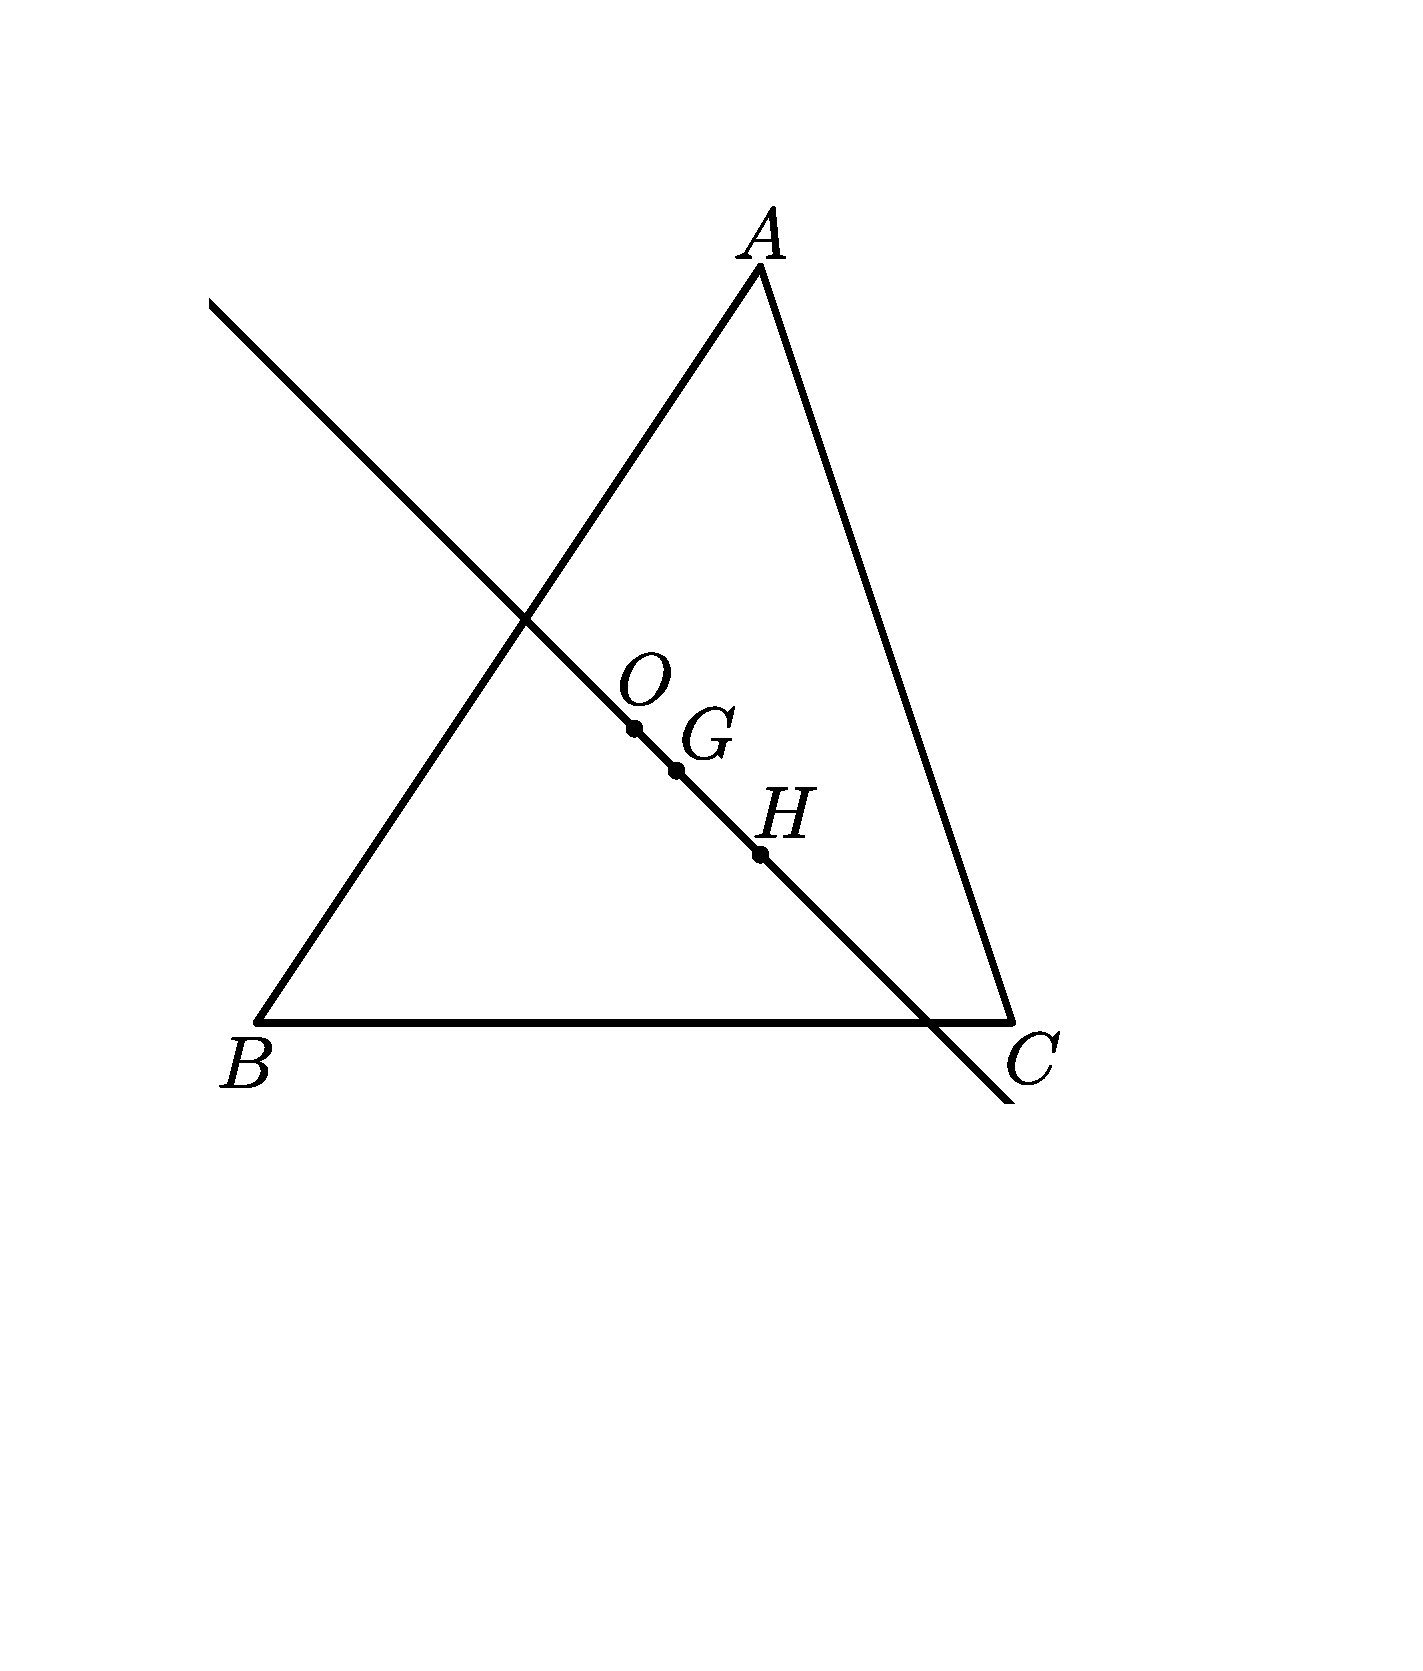
\includegraphics[clip,height=5cm]{figures/Euler.pdf}

\subsection{九点円}
三角形において、各辺の中点と垂線の足、垂心と各頂点の中点は同一円周上にあり、その円を九点円という。

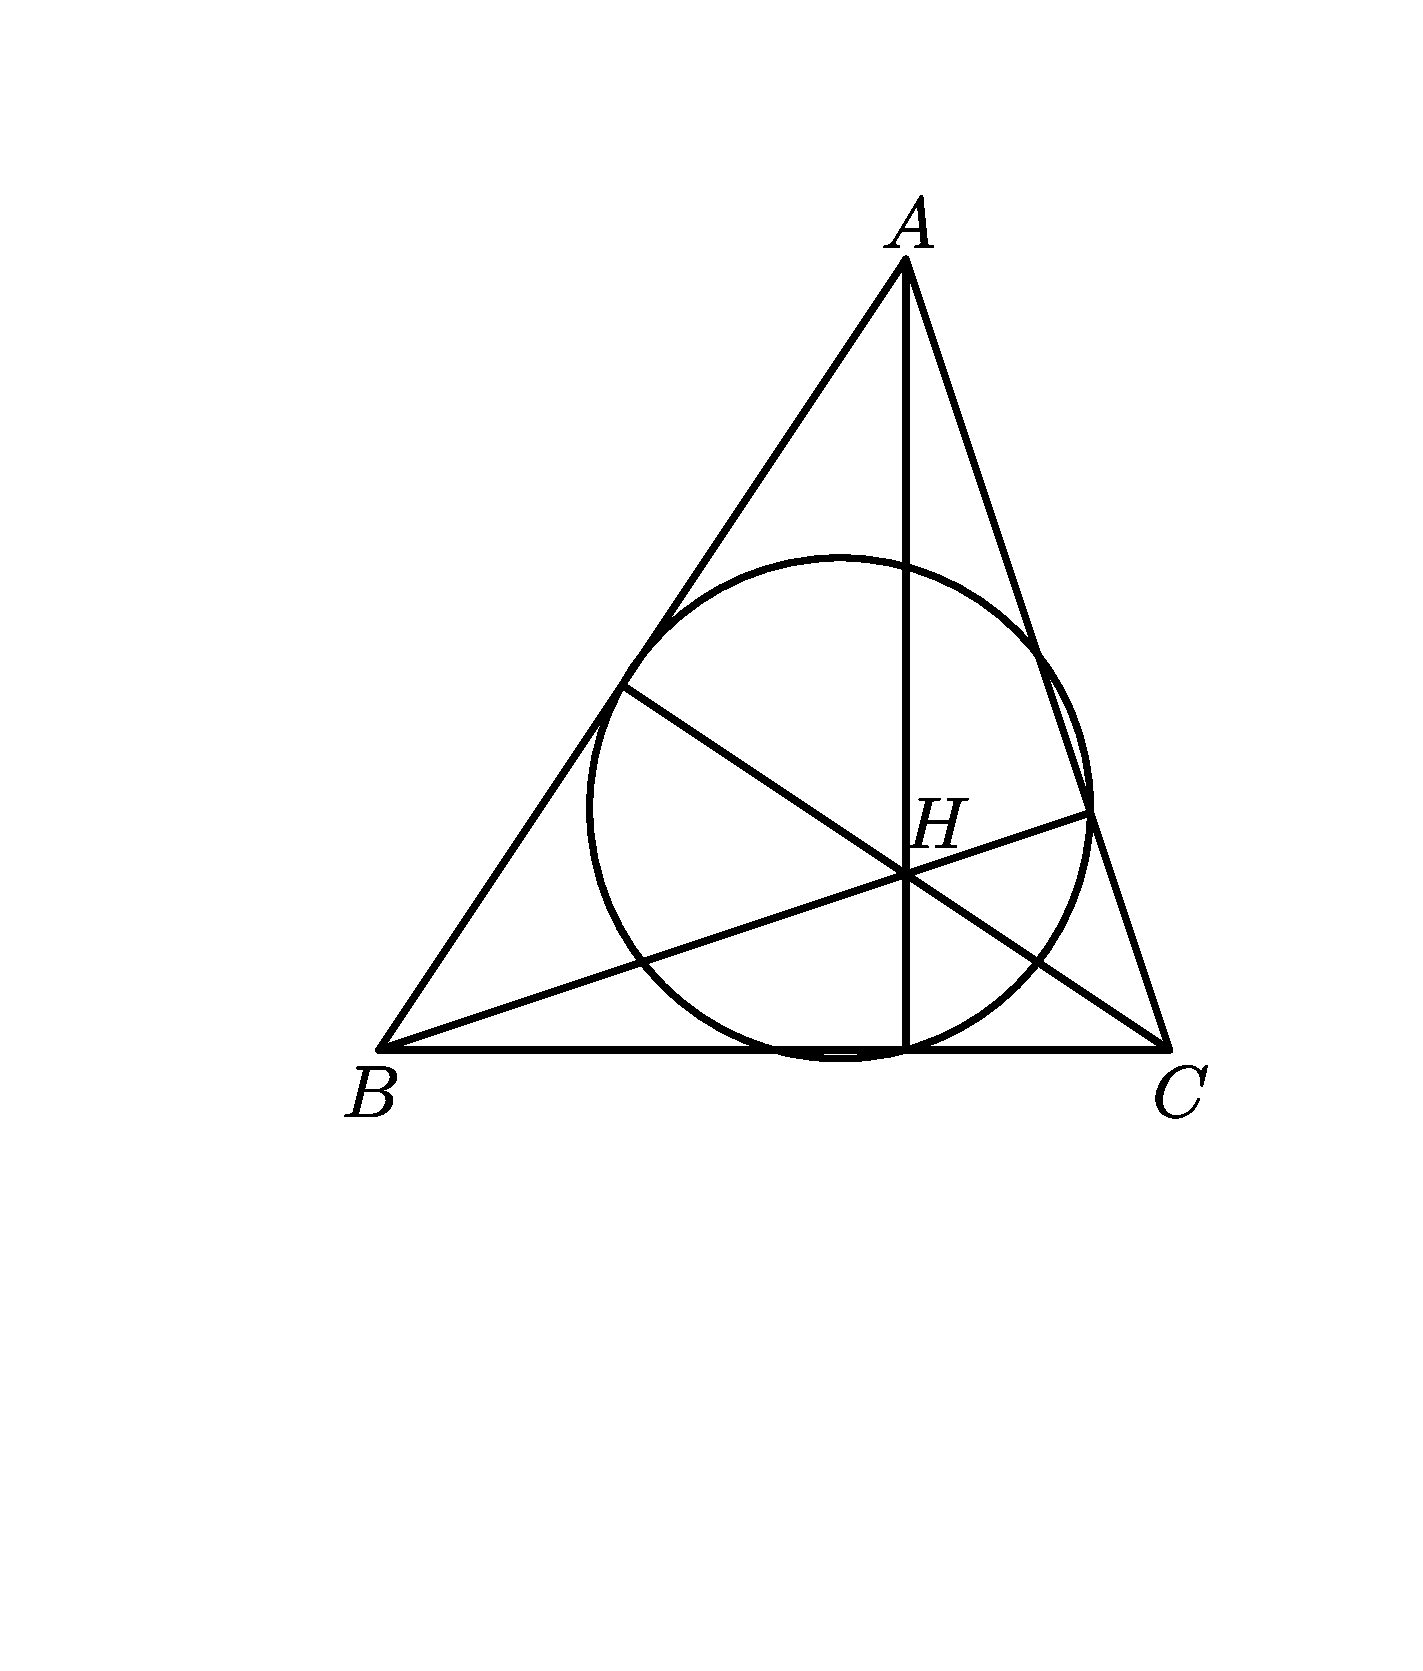
\includegraphics[clip,height=5cm]{figures/Euler_circle.pdf}

\subsection{反転}
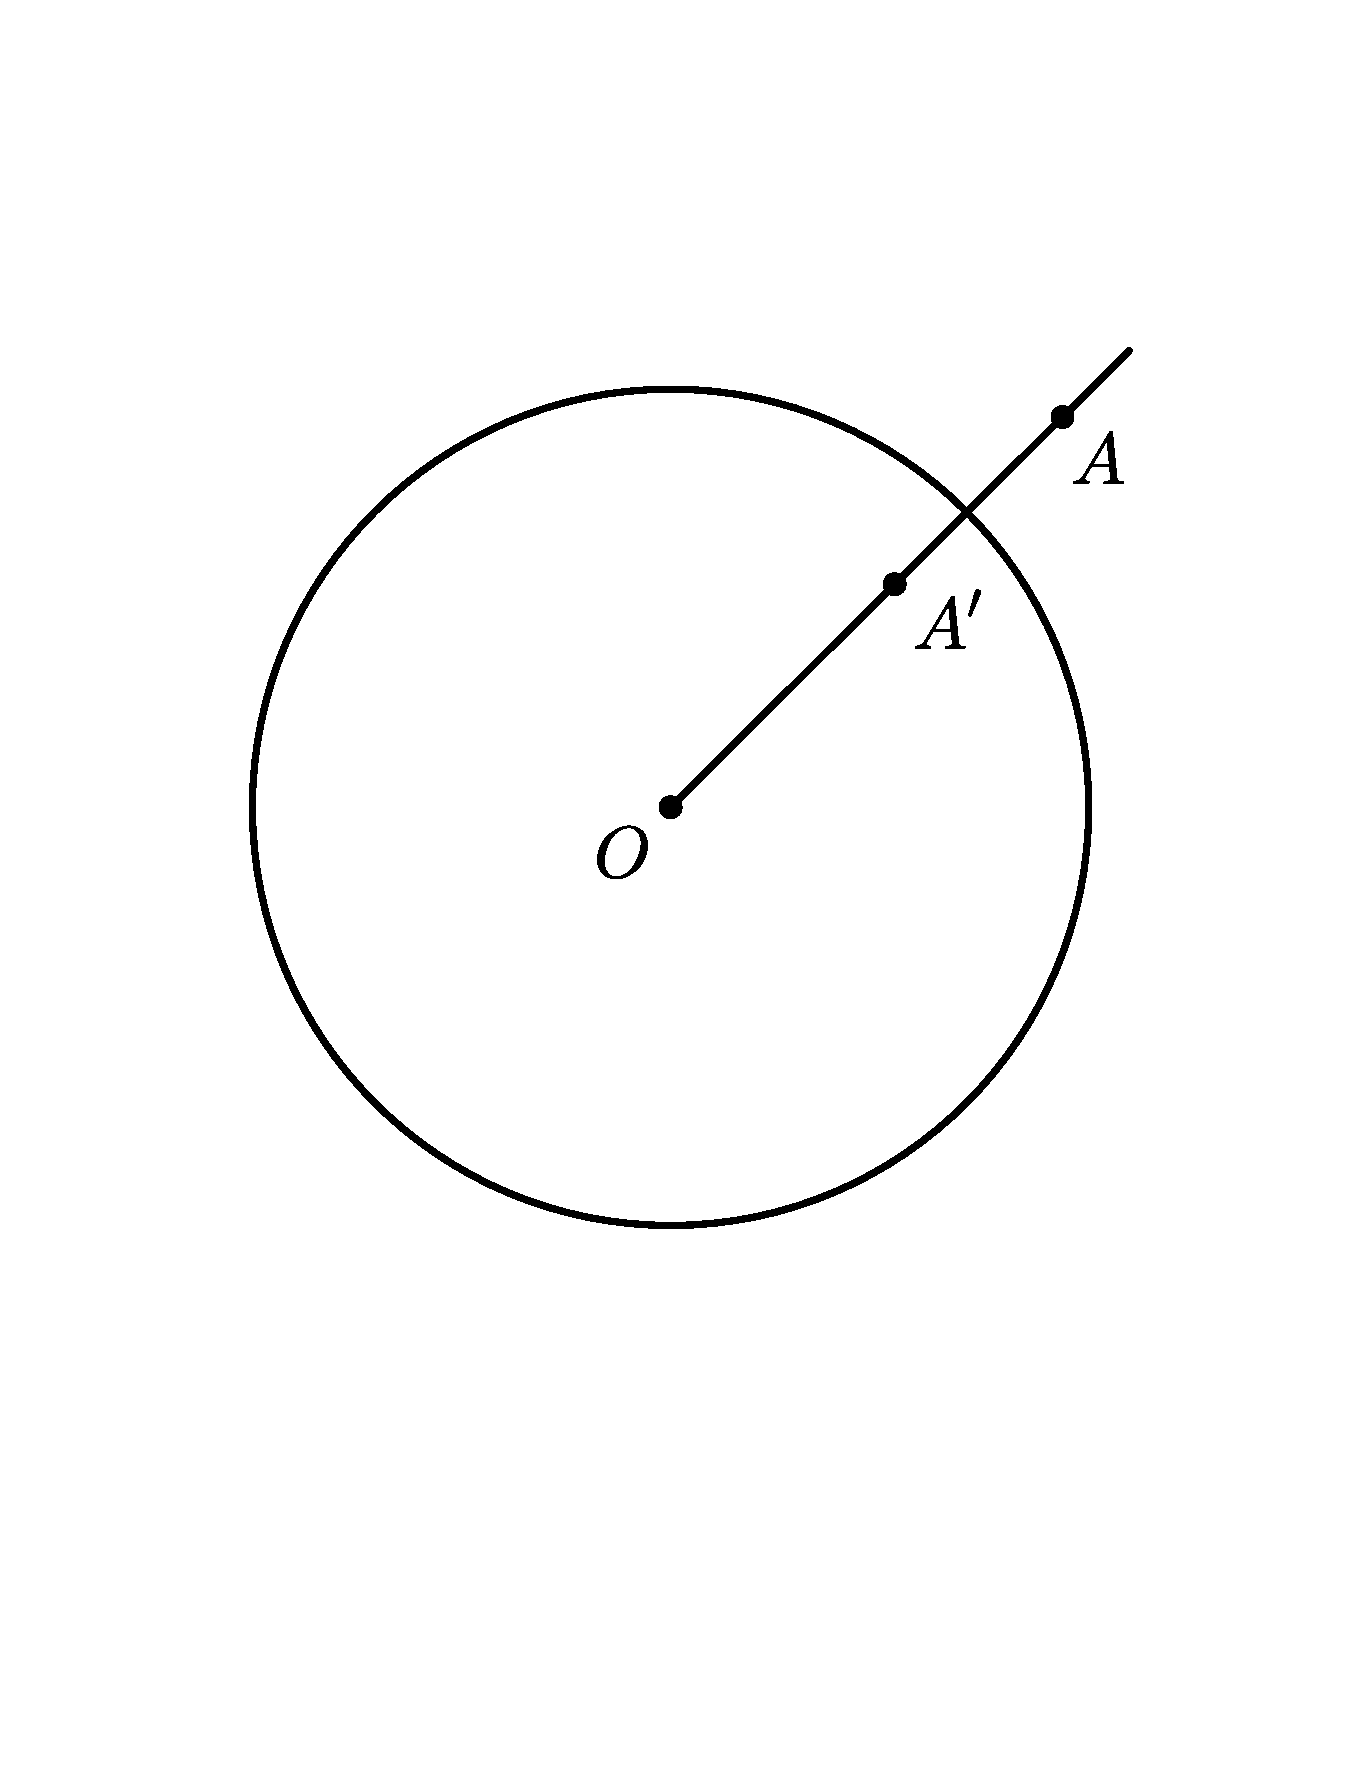
\includegraphics[clip,height=4cm]{figures/Hanten.pdf}

反転とは、円を用いて点の変換を行うものである。中心$O$、半径$r$の円で点$A$を反転するとき、
点$A$を反転した点$A'$は半直線$OA$上の点であり、$\displaystyle OA'=\frac{r^2}{OA}$を満たす。
$O$と一致する点は反転すると無限遠点という仮想の点になると考える。逆に、無限遠点は反転すると、$O$に戻る。
反転を行うと、直線や円は以下のように変換される。
\begin{quote}
    $O$を通らない円$\leftrightarrow$$O$を通らない円

    $O$を通る円$\leftrightarrow$$O$を通らない直線

    $O$を通らない直線$\leftrightarrow$$O$を通る円

    $O$を通る直線$\leftrightarrow$$O$を通る直線(自分自身)
\end{quote}
これらは、直線は無限遠点を含むと考えると、簡単に導出することができる。

反転をしても、図形どうしの交点の数はだいたい変わらず、
図形が接している、接していないという状況は変わらない。
1点を通る円が多いとき、その点を中心とする円で反転すると直線が多くなって図が簡単になる。

\section{三角法}
ここではあまり三角法については触れない。正弦定理、余弦定理が使えれば問題ない。

\section{問題演習}
\subsection{問題を解くうえで}
以下の事項に気を付けながら問題を解く。
\begin{itemize}
    \item コンパスと定規を使った正確な作図を行う。
    \item 図を見て予想を立てる。
    \item 基本事項が使えないか考える。
\end{itemize}
また、この章の最初に紹介した4つの分野を、自分はこれを使うなどと決めず、行き来しながら臨機応変に解くことが大切である。

以下、初等幾何の問題を載せている。解答には図を載せているが、できるだけみないで解くのが好ましい。

\begin{problem}{練習問題1}
    相異なる3点$D,B,C$は同一直線上にあり,$DB=BC=2$である。
    点$A$は$AB=AC$をみたし,直線$AC$と直線$DC$にそれぞれ$A,D$で接する円$\Gamma$が存在する。
    $\Gamma$と直線$AB$の交点のうち$A$でない方をEとし,直線$CE$と$\Gamma$の交点のうち$E$でない方を$F$とするとき,
    線分$EF$の長さを求めよ。

    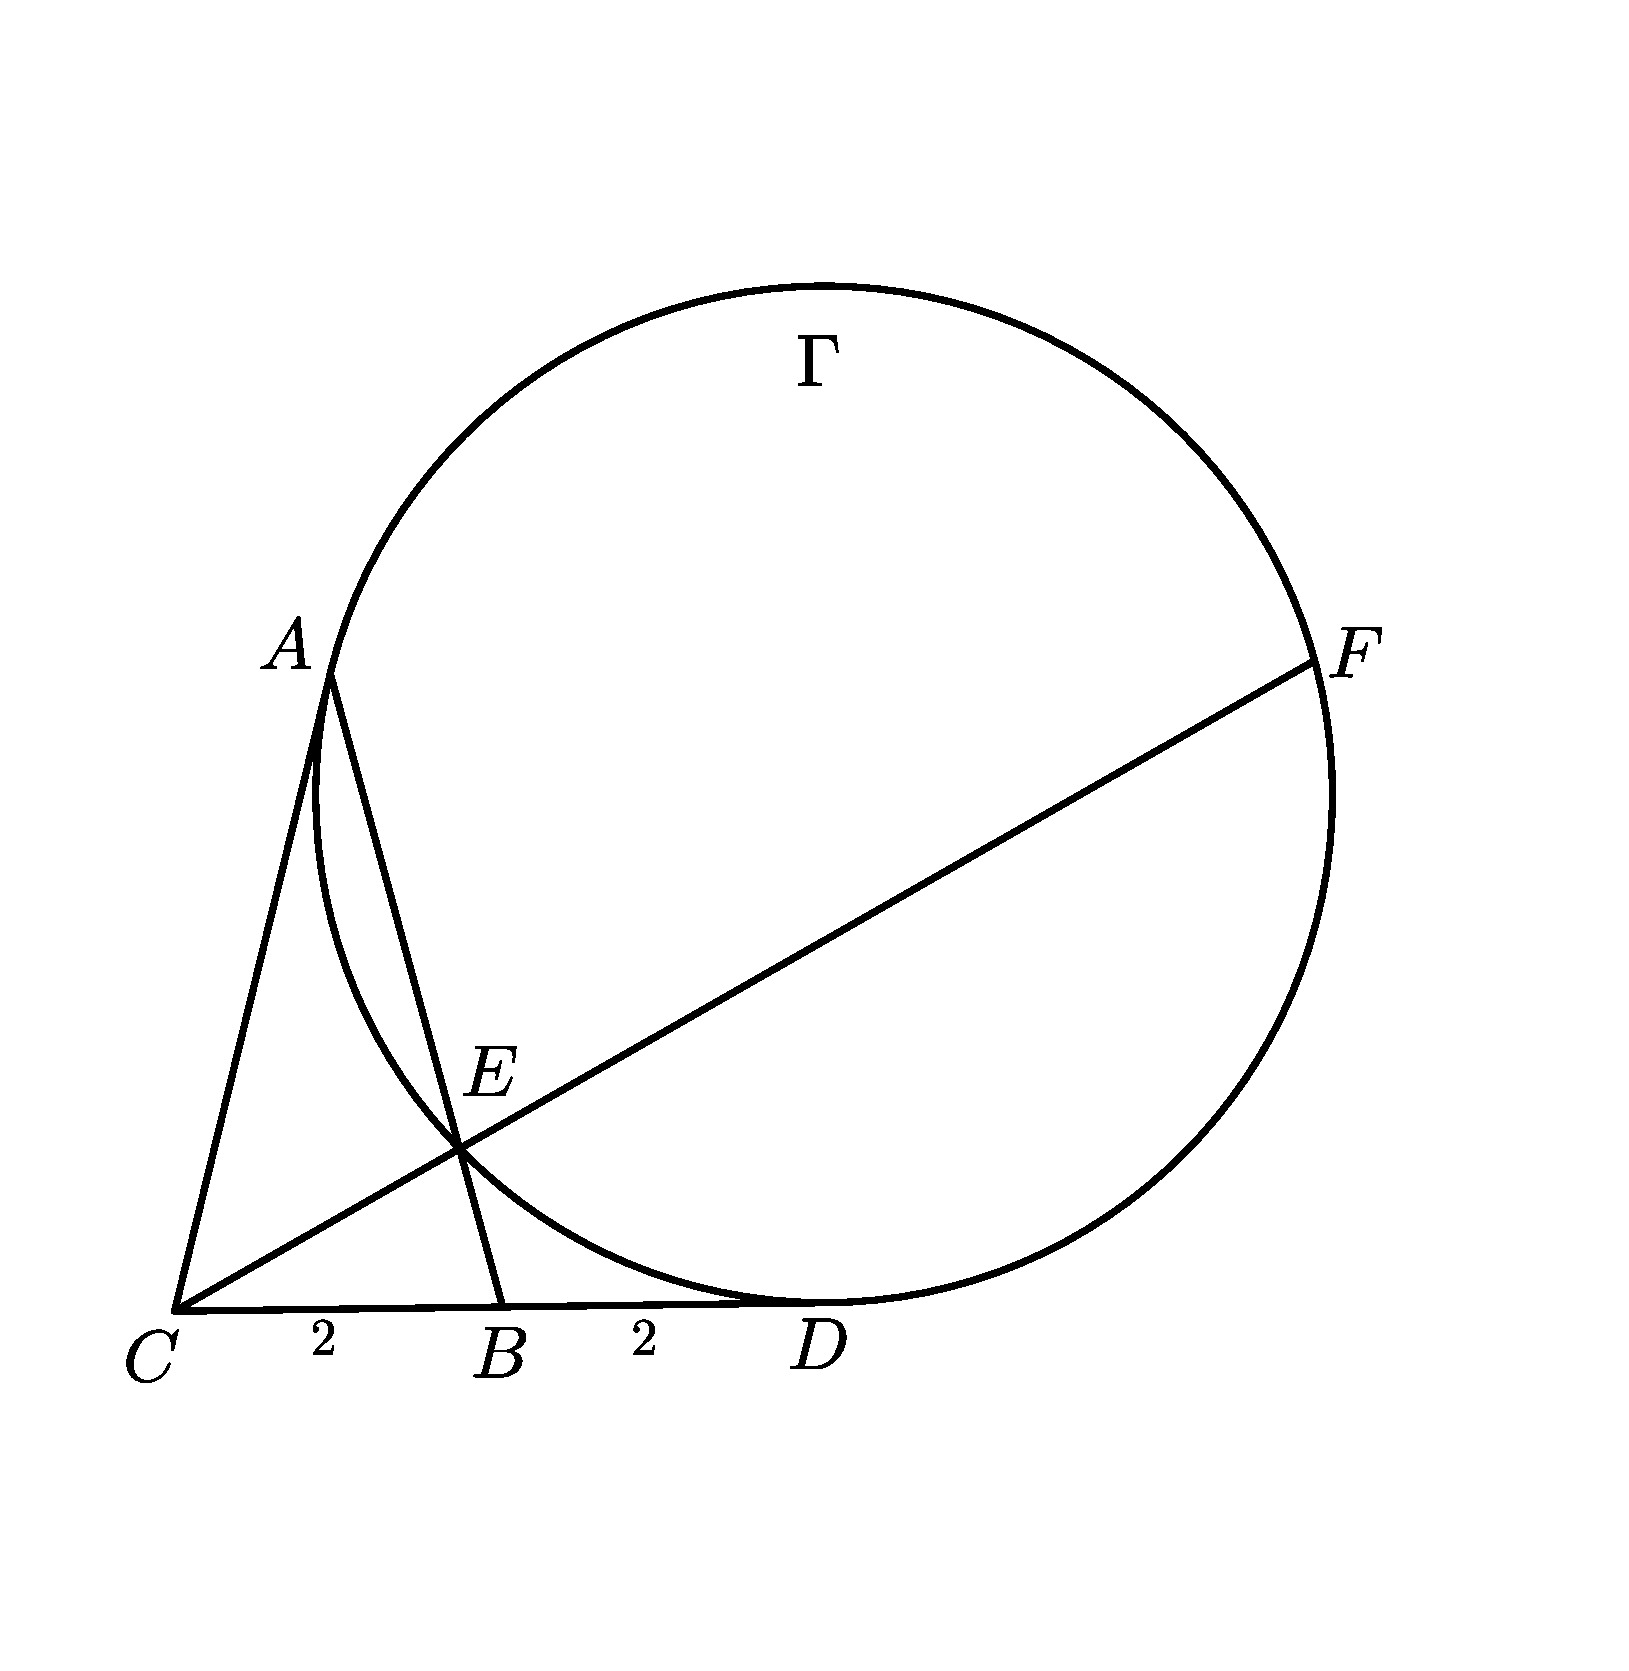
\includegraphics[clip,height=5cm]{figures/practice1.pdf}

\end{problem}

\paragraph{ポイント} 何がわかったら答えが出るのか、逆算しながら考える。

\begin{answer}
    方べきの定理より、$CE\times CF=CD^2$であるから、$CE$がわかれば$CF$が求まるので、方針として$CE$の値を考える。

    $CA$と$CD$は共に$\Gamma$の接線であるから、

    $CA=CD=4$

    仮定より、

    $AB=AC=4$

    方べきの定理より、

    $BE\times BA=BD^2$

    $BE(4-BE)=4$

    $BE=4$

    よって

    $AB:BC=CB:BE=2:1$

    $\angle ABC = \angle CBE(\because 共通)$

    であるから、

    $\triangle ABC ∽ \triangle CBE$

    相似比は$2:1$だから、

    $\displaystyle CE=\frac{1}{2}AB$

    $=2$

    方べきの定理より

    $CE\times CF = CD^2$

    $2(EF+2)=16$

    $EF=6$
\end{answer}

\begin{problem}{練習問題2}
    三角形$ABC$で、$\angle A=60^\circ,angle B=20^\circ,AB=1$のとき、
    $\displaystyle\frac{1}{AC}-BC$の値を求めよ。
\end{problem}

\paragraph{ポイント} $20^\circ$という角は非常に扱いにくいので、うまく補助線を引く。

\begin{answer}
    $AC=x,AB=y$とおく。

    $20^\circ$という角は非常に扱いにくいので、以下のように補助線を引いて正三角を作る。

    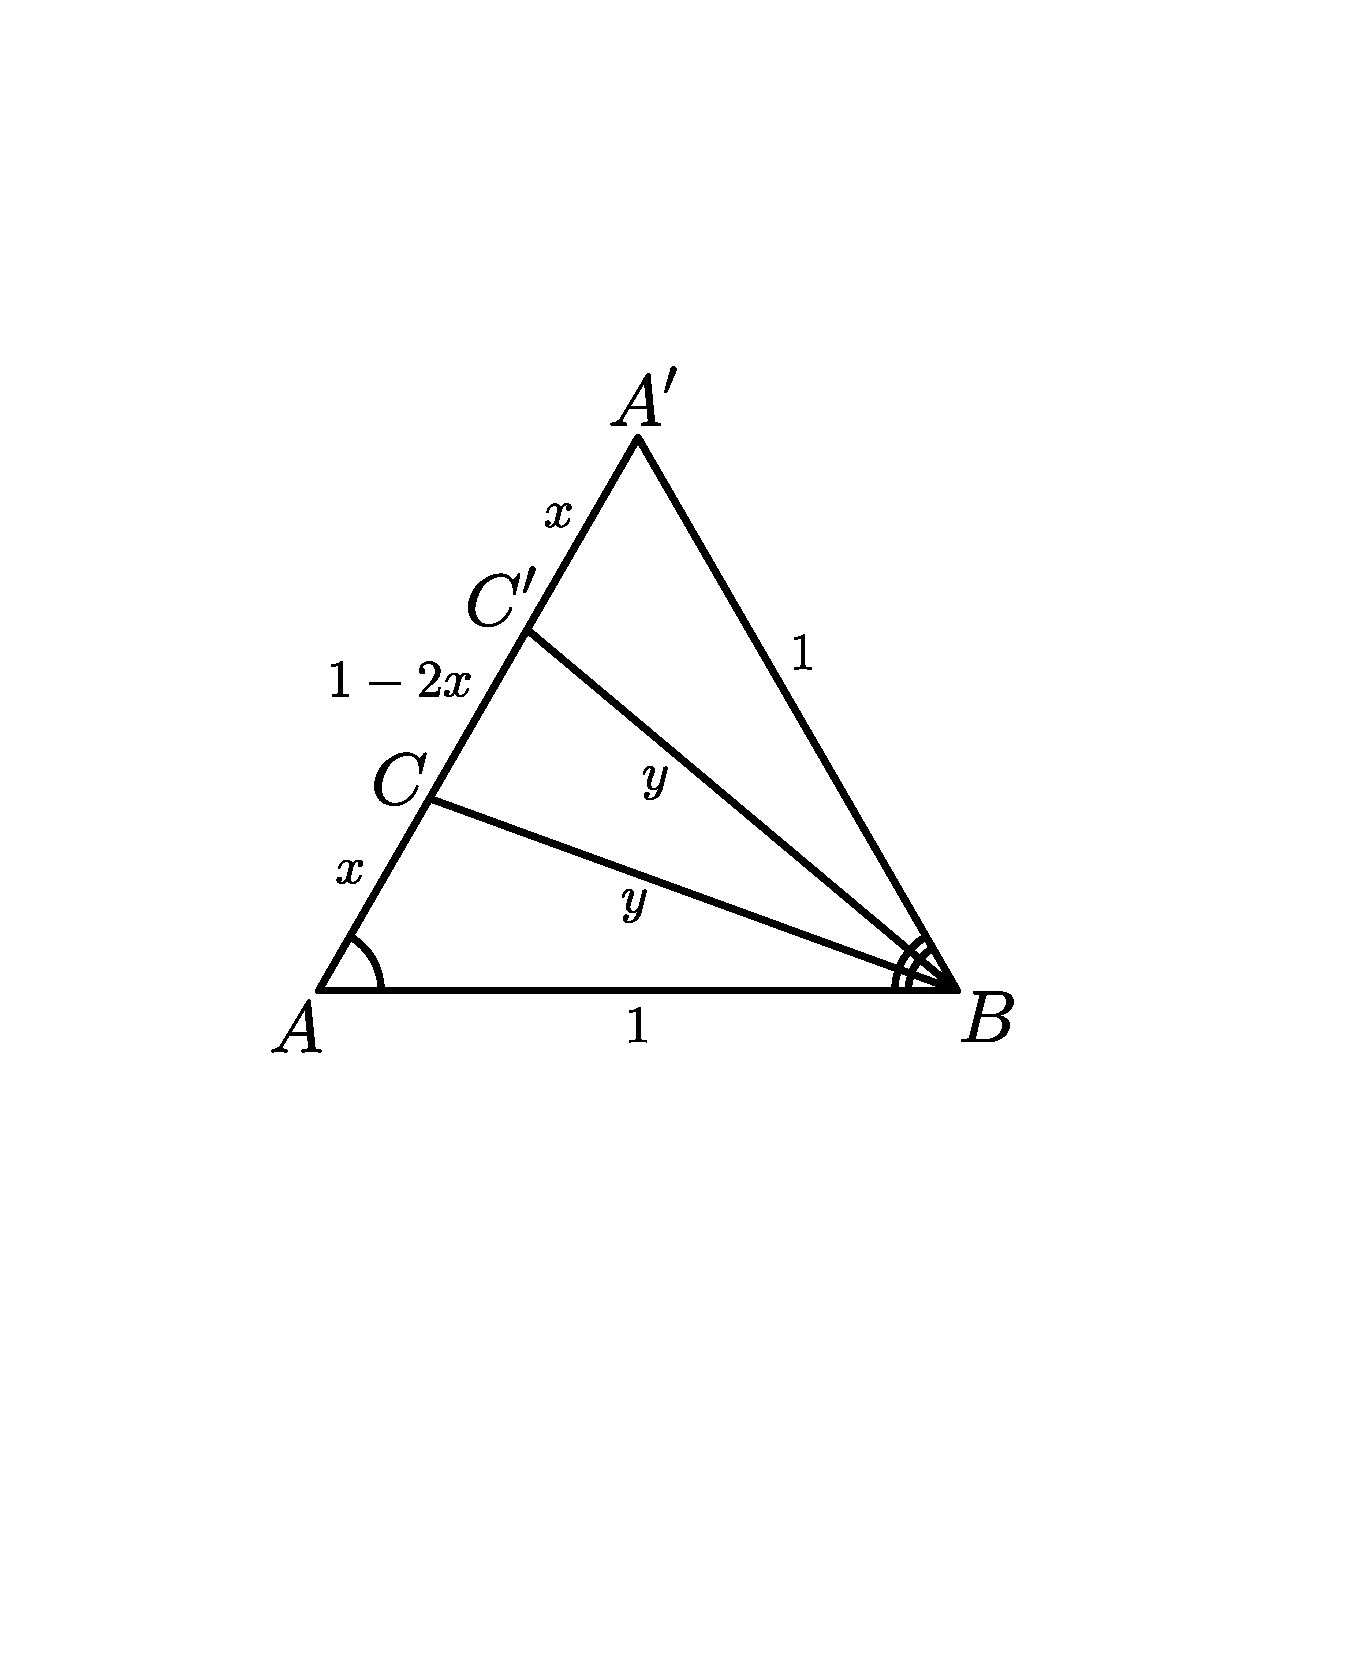
\includegraphics[clip,height=5cm]{figures/practice2.pdf}

    $\triangle ABC'$に着目すると、

    $BC$は$\angle ABC'$の二等分線だから、

    $AB:BC'=AC:CC'$

    $1:y=x:(1-2x)$

    $\displaystyle y = \frac{1}{x}-2$

    $\frac{1}{x}-y=2$

    $\therefore 2$
\end{answer}

次の問題は、作図をするところから頑張って欲しい。

\begin{problem}{練習問題3}
    $\triangle ABC$は、$AB=AC$の二等辺三角形である。

    $\triangle ABC$の外接円の、$C$を含まない弧$AB$上に、点Fを取る。

    $\triangle ABC$の外接円の$B$における接線$l$と、直線$AF$の交点を$K$、
    直線$AB$と直線の$CF$の交点を$L$とするとき、
    4点$F,L,B,K$は同一円周上にあり,$KL$と$BC$は平行であることを示せ。
\end{problem}

\begin{answer}
    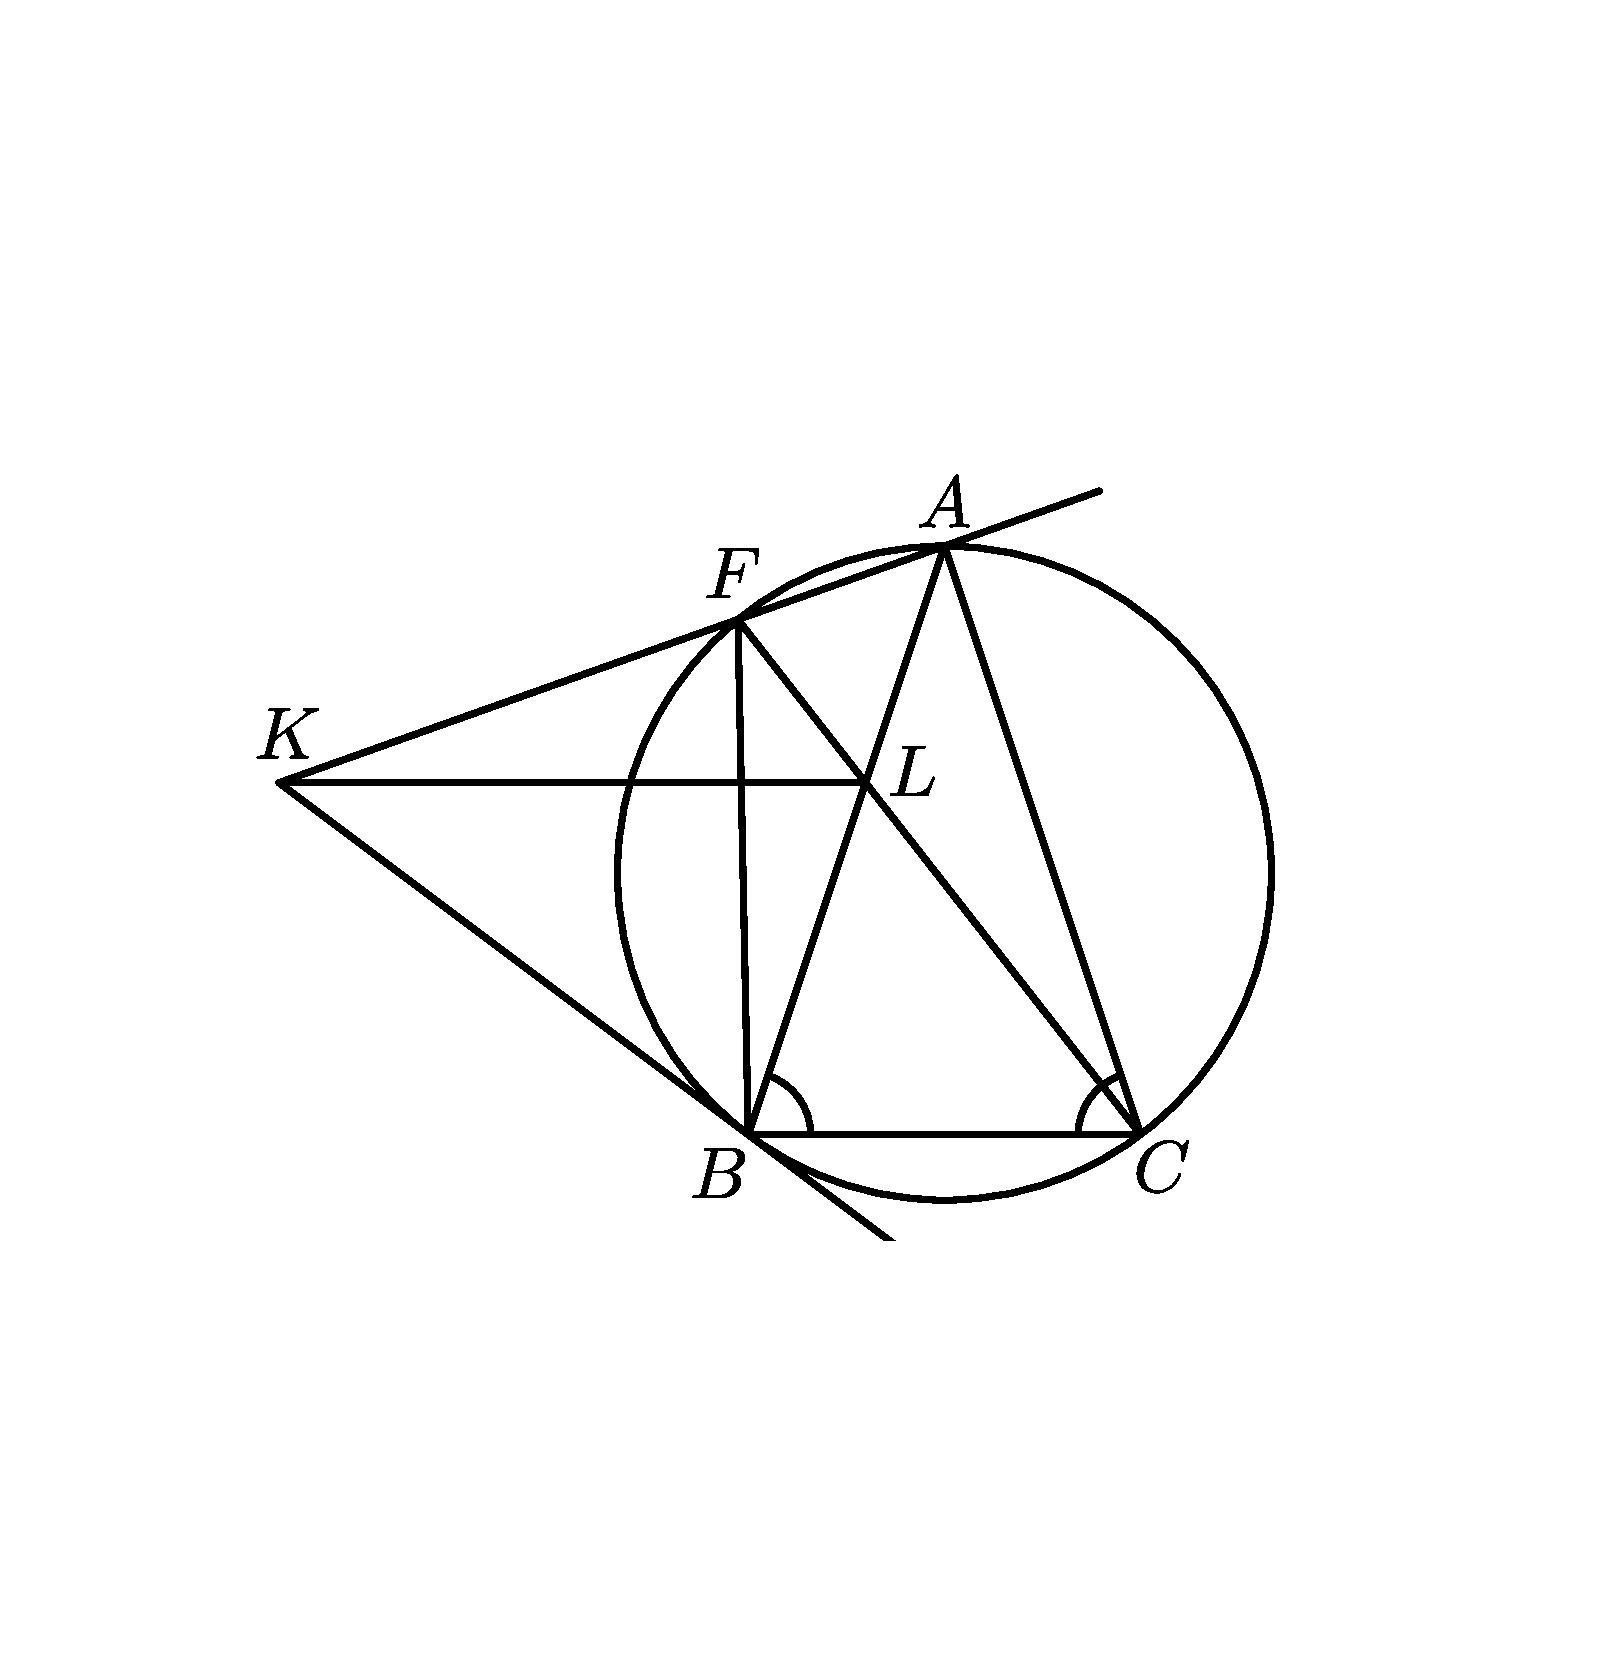
\includegraphics[clip,height=5cm]{figures/practice3.pdf}

    接弦定理より、

    $\angle KBL=\angle ACB$

    $\triangle ABC$は、$AB=AC$の二等辺三角形だから、

    $\angle ACB=\angle ABC$

    円周角の定理より、

    $\angle ABC=\angle AFC$

    よって$\angle KBL=\angle AFC$であるから、

    $F,L,B,K$は同一円周上にある。

    四角形$FBCA$は円に内接するから、

    $\angle ACB=\angle KFB$

    $F,L,B,K$は同一円周上にあるから、円周角の定理より

    $\angle KFB=\angle KLB$

    よって$\angle KLB=\angle ABC$となり、
    錯覚が等しいから$KL$と$BC$は平行。
\end{answer}
この解法は非常にシンプルであり、思いつかないと思うかもしれないが、
Angle-chaseをひたすらすれば多少ごちゃごちゃしてしまっても解ける。
記述が大変だが、一つの良い手である。

\begin{problem}{練習問題4}
    下の図において、

    $OA=5,OB=6,OC=20$

    $AC\perp BD$

    である。

    4つの円すべてに接する円が存在するとき、$OD$の長さを求めよ。

    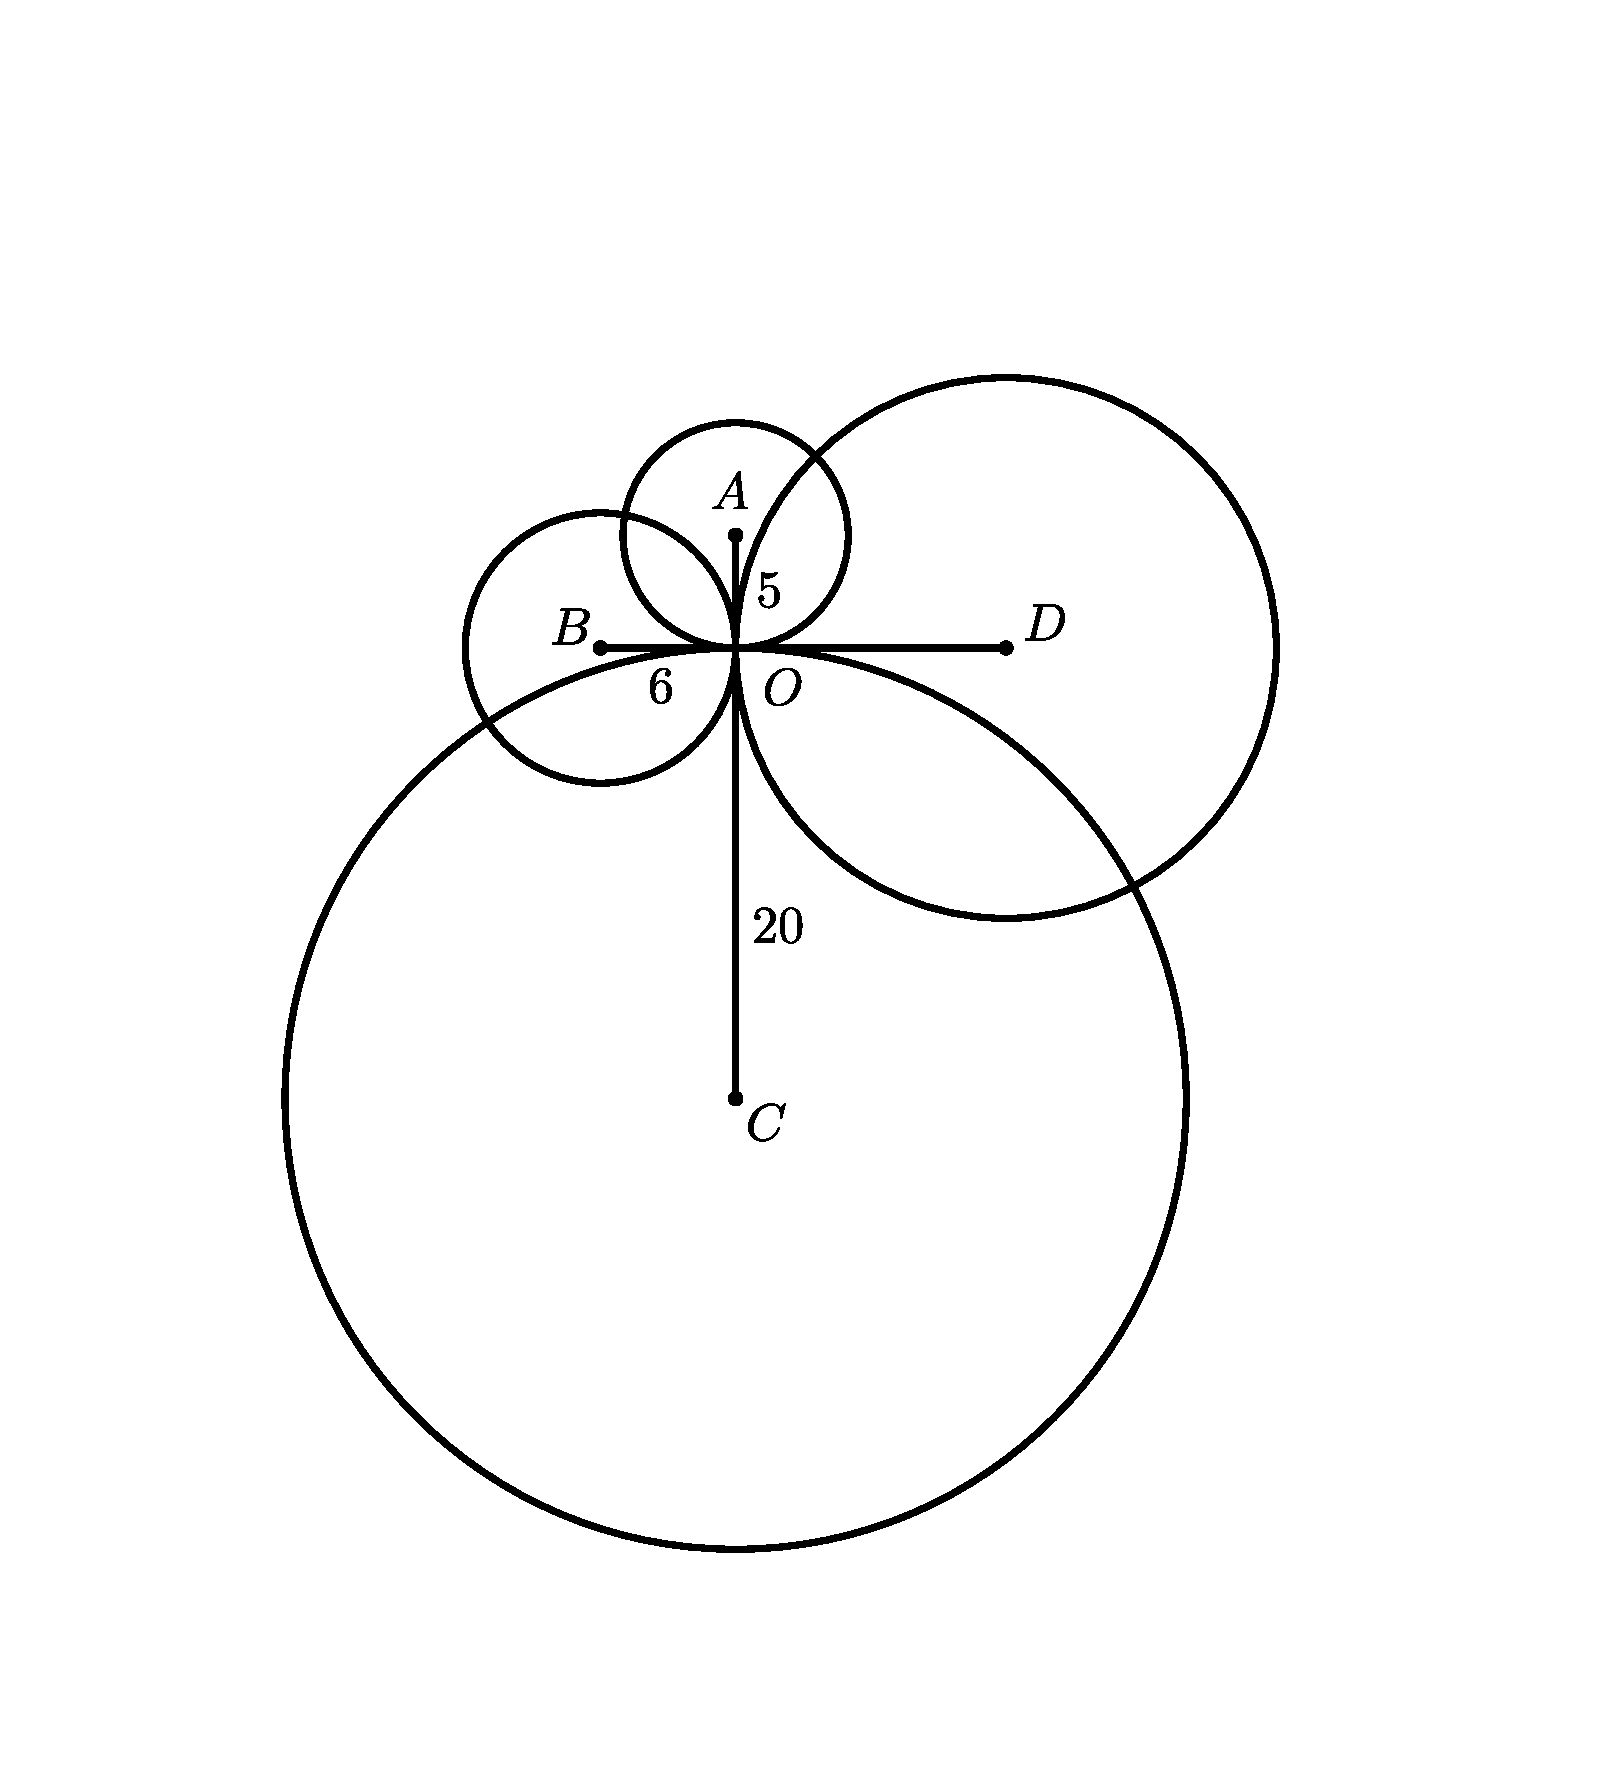
\includegraphics[clip,height=5cm]{figures/practice4.pdf}
\end{problem}

\paragraph{ポイント}$O$を中心とする円で反転をすると、4つの円がすべて直線になる。

\begin{answer}
    $OD=x$とおく。

    4つの円を中心$O$、半径$1$の円で反転すると、図のようになる。

    4つの円に接する円は$O$を通らないので、同様に反転すると、円になる。

    4つの円を反転した図形それぞれに接する円を書くことができれば良いので、

    図の四角形が正方形になれば良い。

    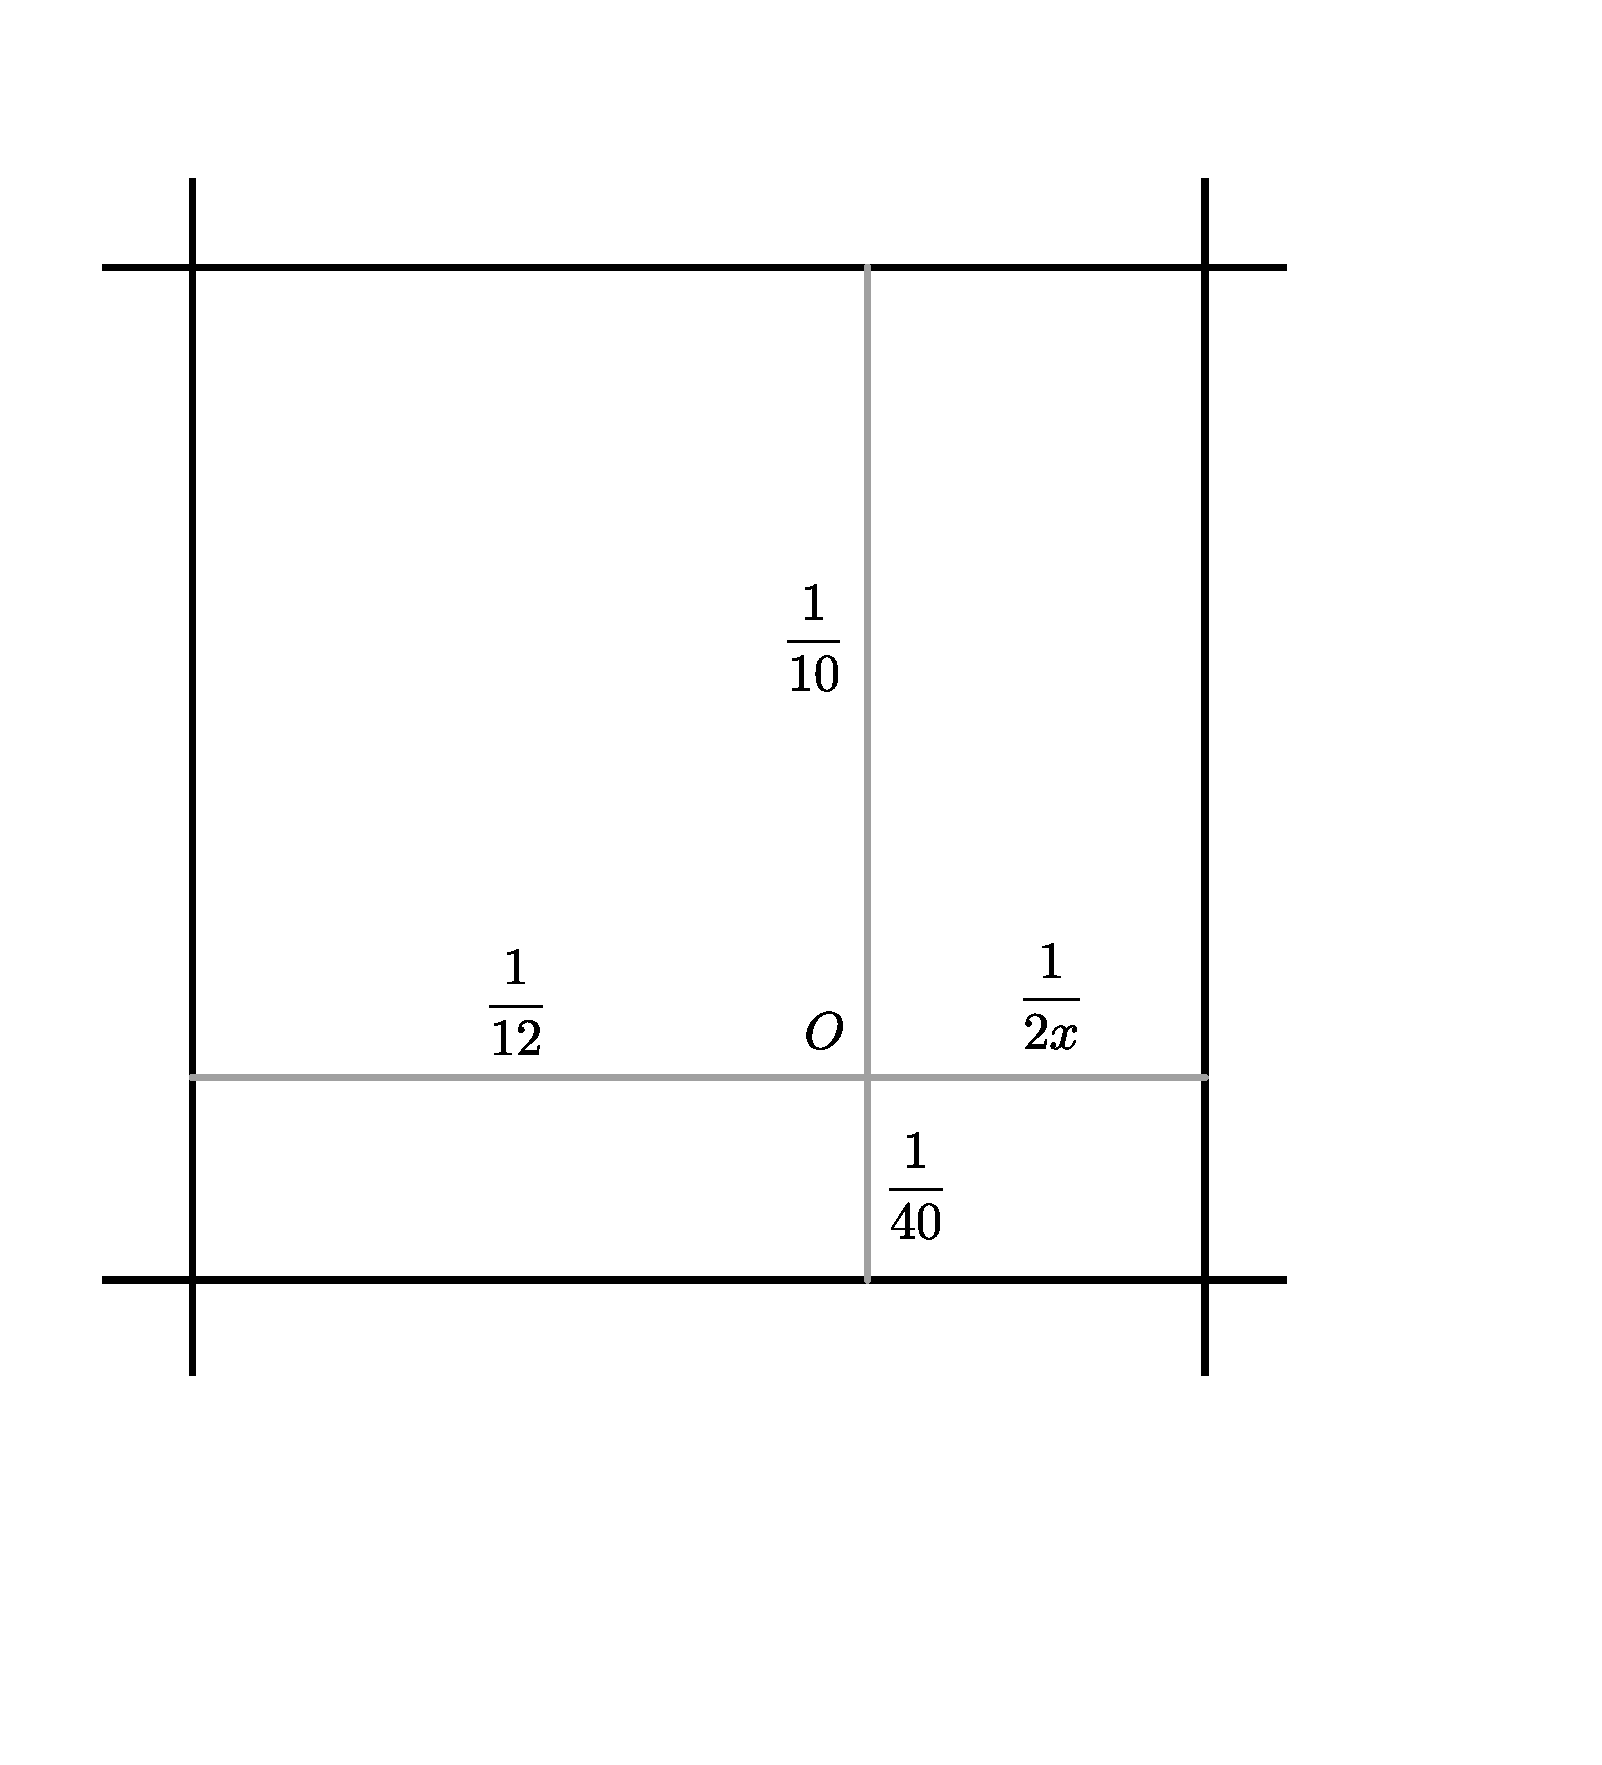
\includegraphics[clip,height=5cm]{figures/practice4_ans.pdf}

    $\frac{1}{2x}+\frac{1}{12}=\frac{1}{10}+\frac{1}{40}$

    $x=12$

    $\therefore 12$
\end{answer}

\chapter{組み合わせ}
学校で習う組み合わせと競技数学での組み合わせは少し異なる。
学校では主に何通りあるかや確率を求めよなどの問題が出される。
競技数学における組み合わせは、様々な考え方を駆使して解くものであり、統一的な解き方がない。
基本的には小さい値で実験して考える。
うまい発想により一発で解けることが多いが、そうでないと解けないことがあり、まさに運ゲーである。

問題を解く上で大切なこととして、以下の2つが挙げられる。
\begin{quote}
    \begin{description}
        \item[①]良い言い換えを見つける
        \item[②]問題をシンプルにする
    \end{description}
\end{quote}

①の例として、以下の練習問題を解いて欲しい。

\begin{problem}{練習問題}
    図のようにぶら下がっている8個の的を1回ずつ撃つ。
    下にまだ撃たれていない的がある場合、その的は撃つことができない。
    8個の的の撃ち方は何通りか。ただし、狙った的は確実に撃てるものとする。

    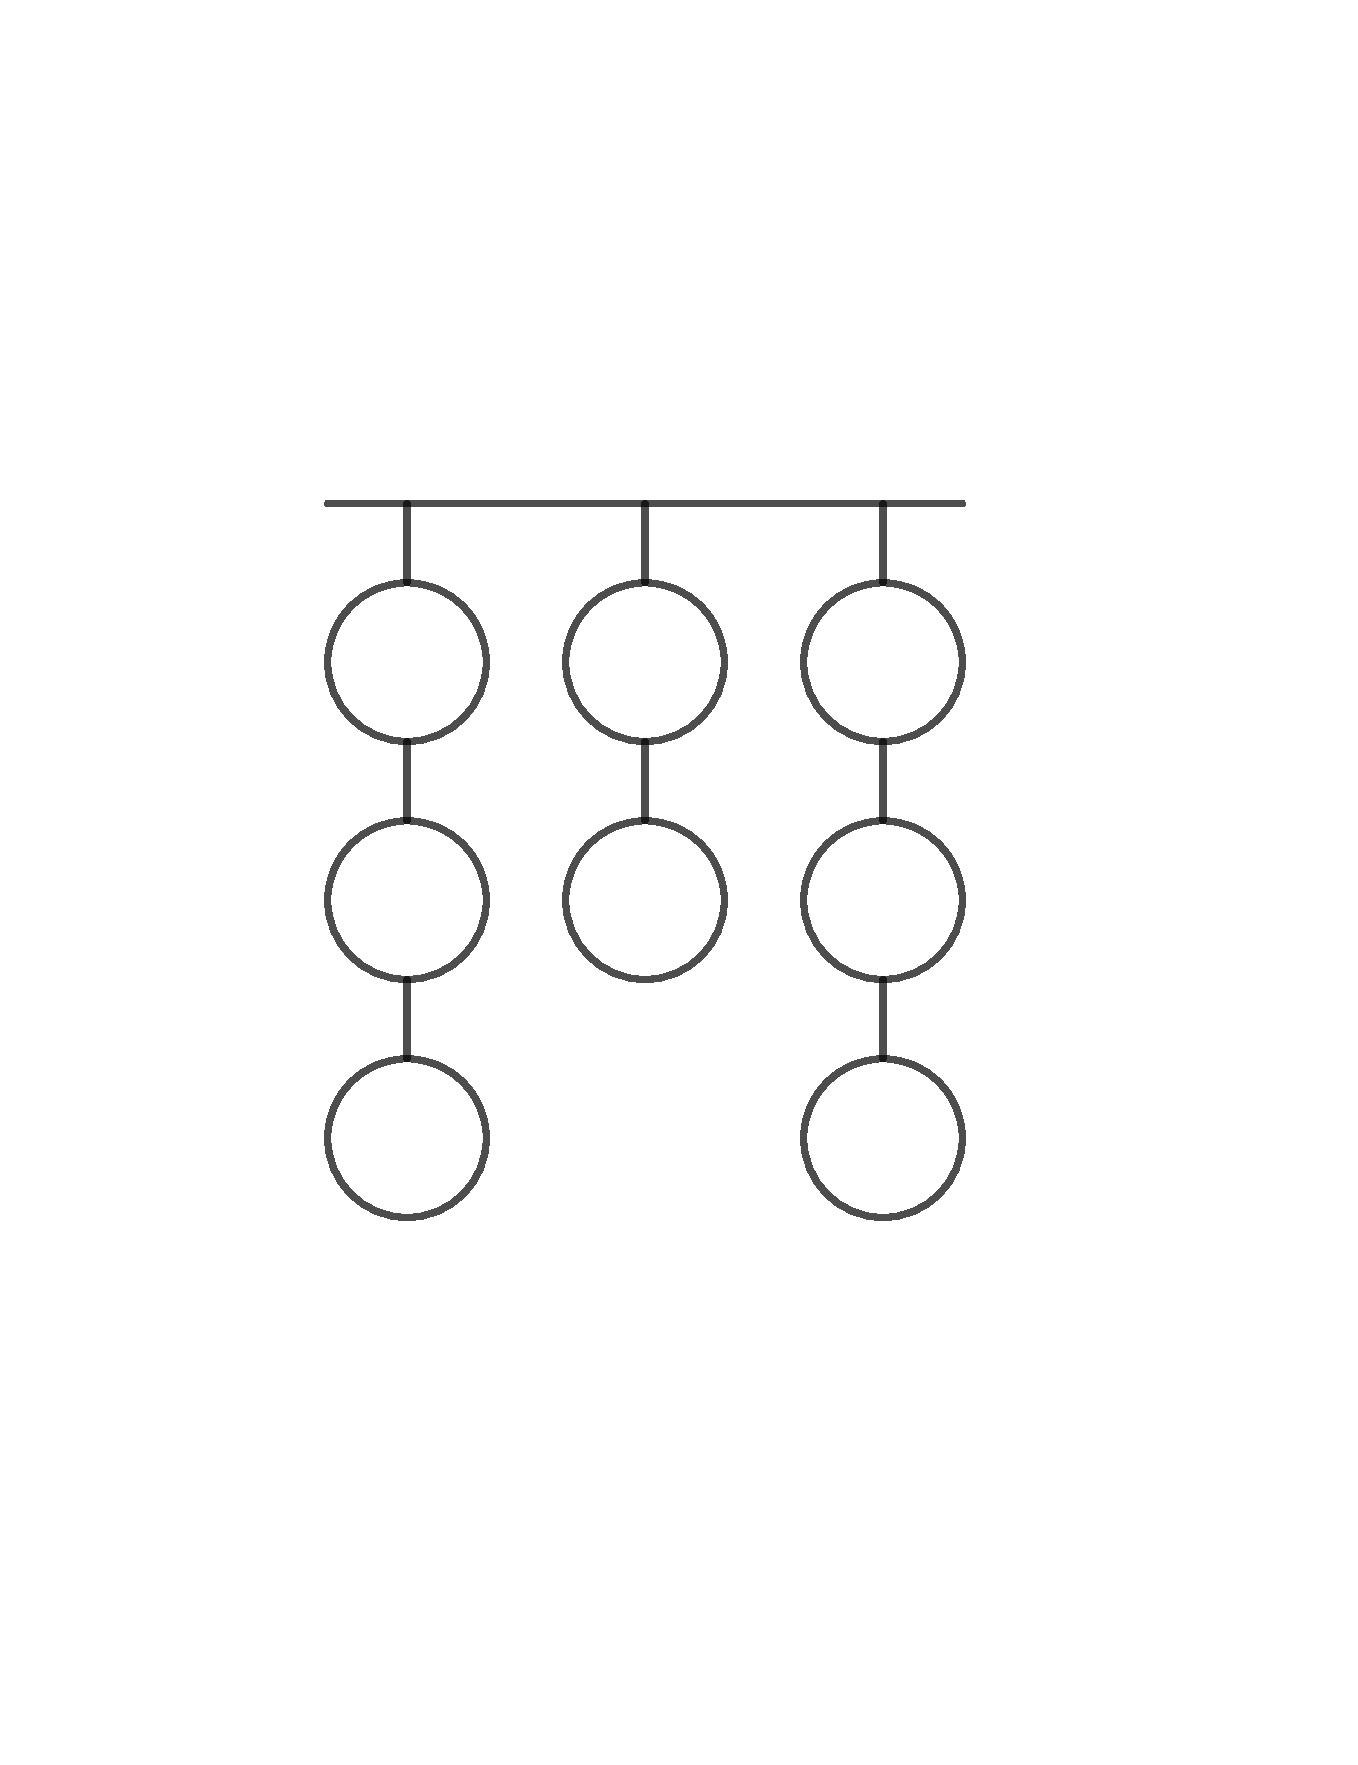
\includegraphics[clip,width=2cm]{figures/c_practice1.pdf}
\end{problem}

\begin{answer}
    この問題は、文字の並べ替えの問題に言い換えることができる。

    3文字のA、2文字のB、3文字のCでできた文字列を考える。
    文字列の左から順に、Aがあったら左にぶら下がっている的で撃たれていないもののうち一番下、Bがあったら左にぶら下がっている的で撃たれていないもののうち一番下、Cがあったら左にぶら下がっている的で撃たれていないもののうち一番下を撃つようにすれば良い。

    3文字のA、2文字のB、3文字のCの並べ方は、

    ${}_8\mathrm{C}_3 + {}_5\mathrm{C}_2 + {}_3\mathrm{C}_3
    =560(\text{通り})$

    $\therefore 560$通り
\end{answer}

\section{組み合わせ}
ここでは学校でやるような組み合わせの問題を取り上げる。
\begin{problem}{練習問題1}
    7つの席が横一列に並んでおり、7人が1人ずつ順番に座る。
    ただし、隣に人が座っていない席がある場合、その席に優先的に座っていく。
    このとき、座る順番は何通りあるか。
\end{problem}
\paragraph{ポイント}この問題は条件が難しく、数え上げなければならない。工夫して数え上げよう。

\begin{answer}
    途中で隣に他人が座っている席に座らなければならない人が出てくる。
    隣に人がいない席に座れた人を○、座れなかった人を×で表すと、○と×の並び順は以下の7通り。

    \begin{tabular}{|ccccccc|}
        \hline
        ○ & × & ○ & × & ○ & × & ○\\\hline
        ○ & × & ○ & × & × & ○ & ×\\\hline
        ○ & × & × & ○ & × & ○ & ×\\\hline
        ○ & × & × & ○ & × & × & ○\\\hline
        × & ○ & × & ○ & × & ○ & ×\\\hline
        × & ○ & × & ○ & × & × & ○\\\hline
        × & ○ & × & × & ○ & × & ○\\\hline
    \end{tabular}

    ○が4つの場合、座り方は$4!\times 3!$通り。

    ○が3つの場合、座り方は$3!\times 4!$通り。

    求める場合の数は、

    $7\times 4!\times 3!=1008(通り)$
\end{answer}

\begin{problem}{練習問題2}
    1から13までの数字が1つずつ書かれた13枚のカードがある。
    カードを裏返しにして横一列に並べ、左から順にめくる。
    めくったカードがそれまでめくった中で最大でなければそのカードを捨てる。
    このとき、7が残っている確率はいくらか。
\end{problem}

\paragraph{ポイント}きちんと考えれば解くことができるが、発想により一発で解くことができる。

\begin{answer}
    書かれた数字が7以上である7枚のカードのうち、最初のカードが7であれば良いので、$\displaystyle\frac{1}{7}$
\end{answer}

\begin{problem}{練習問題3}
    表にA、裏にBと書いてあるコインがある。12回投げて、連続する2回の記録を全て取ったところ、以下のようになった。

    \begin{tabular}{cc}
        AA & 2回\\
        AB & 3回\\
        BA & 2回\\
        BB & 4回\\
    \end{tabular}

    このとき、AとBの出かたの組み合わせは何通りか。
\end{problem}

\begin{answer}
    同じ文字が連続している部分を1文字のみに置き換えると、(例えばAABABBはABABと置き換えられる)
    ABが3回、BAが2回出ていることから、ABABABとなる。
    この文字列のAの部分にAをあと2文字、Bの部分にBをあと4文字追加すればよい。
    Aを追加できる部分は3箇所あり、そこに2文字のAを追加する方法は、2個の○と2本の仕切りの並べ方と1対1対応するので、${}_4{C}_2$通り。同様に、Bを追加する方法は、${}_6{C}_4$通り。

    よって求める組み合わせは、

    ${}_4{C}_2 \times {}_6{C}_4=90$(通り)
\end{answer}

\section{鳩の巣原理}
$n$個の巣箱があり、そこに$n+1$羽の鳩を入れようとすると、少なくとも1つの巣箱には2羽以上の鳩が入らなければならない。これを鳩の巣原理という。これは当たり前のことであるが、とても重要である。問題を解く時には、鳩、つまりグループ分けをするものと巣箱、つまり分けるグループを何にするかを考えることが重要であり、難しい部分である。

\begin{problem}{練習問題1}
    座標平面上に5個の格子点($x$座標、$y$座標が共に整数である点)があり,
    それらの中点は10個ある。中点のうち少なくとも1つは格子点であることを示せ。
\end{problem}

\begin{answer}
    中点が格子点になるのは、$x$座標と$y$座標の偶奇がそれぞれ一致する時である。
    偶奇の組み合わせは4通りであり、格子点は5個であるから、鳩の巣原理より、座標とy座標の偶奇がそれぞれ一致する点が少なくとも1つ存在する。
    よって題意を満たす。
\end{answer}

\begin{problem}{練習問題2}
    1から9の数字が20個並んでいる数列がある。
    連続する部分の積のうち、平方数になるものが必ず存在することを示せ。
\end{problem}

\paragraph{ヒント}最初から$n$番目$(n=1,2,\dots,20)$までの積を並べた数列を考え、ある整数$i,j( 1 \leqq i < j \leqq 20 )$について、その数列の$j$番目を$i$番目で割った値が平方数になれば良い。

\begin{answer}
    最初から$n$番目$(n=1,2,\dots,20)$までの積を並べた数列を考える。ある整数$i,j( 1 \leqq i < j \leqq 20 )$について、その数列の$j$番目を$i$番目で割った値が平方数になれば良い。
    ある数が平方数であるには、その数を素因数分解した時に、指数が全て偶数であれば良い。
    元の数列は1以上9以下の数が並んだものだから、積を並べた数列のうち、$2,3,5,7$の指数の偶奇が一致する項が存在すれば良い。
    指数の偶奇は$2^4=16$通り。
    鳩の巣原理より、20個の積のうち、少なくとも1組は指数の偶奇が一致する。
    よって連続する部分の積のうち、平方数になるものが必ず存在する。
\end{answer}

\subsection{パズルゲーム}

パズルゲームの問題では、マス目を色分けするような問題がよく出る。

\begin{problem}{例題}
    $1\times 2$のドミノがある。
    $6\times 6$のマスにドミノを敷き詰めることはできるが、
    $5\times 5$のマスにドミノを敷き詰めることはできない。
\end{problem}

\end{document}